\documentclass[10pt,conference]{IEEEtran}
\usepackage{graphicx,booktabs,amsmath,amssymb,array,multirow,microtype,url,xcolor}
\usepackage[T1]{fontenc}
\graphicspath{{../figures/}}
\newcommand{\dyn}{\mathrm{dyn}}
\newcommand{\stat}{\mathrm{stat}}
\newcommand{\logit}{\operatorname{logit}}
\newcommand{\sigmoid}{\operatorname{sigmoid}}
\newcommand{\E}{\mathbb{E}}
\newcommand{\R}{\mathbb{R}}

\title{Source-Aware Evidence Pooling for Dynamic Gaussian Mapping:\\A Reproducible Mechanism Study}
\author{Anonymous Authors}

\begin{document}
\maketitle

\begin{abstract}
Dynamic Gaussian-splatting mapping commonly combines optical flow, geometry, and clustering cues, but derived cues can reuse the same underlying measurements. Treating these channels as conditionally independent can count one source several times and create confidence without new information. We separate this statistical problem from the mapping problem that often accompanies it. First, we define a source-aware logit pool that averages calibrated channels inside each provenance family before combining families. The construction is invariant to uniform replication of all channels within a family. A controlled latent-variable stress test uses ten random seeds, 10,000 calibration samples per seed, and 50,000 disjoint test samples per seed. Replicating one motion channel eight times raises fixed channel-product negative log likelihood from $0.479\pm0.002$ to $1.045\pm0.021$ and expected calibration error from $0.0148\pm0.0019$ to $0.1787\pm0.0020$; the family pool remains unchanged. Second, we isolate dynamic-pixel suppression in a known-pose synthetic Gaussian mapping study. Across 5 independent GPU runs with four held-out views each, static-only initialization plus a masked rendering loss improves static-region PSNR from $27.67\pm0.52$ to $31.70\pm0.23$~dB and reduces dynamic ghost residual from $0.0433\pm0.0089$ to $0.0057\pm0.0002$. Additional capacity and budget sweeps characterize the combined configuration, and matched three-seed tests isolate loss-only masking and fixed false-negative and false-positive mask errors. These are mechanism-level results, not end-to-end SLAM results: the mapping experiment uses oracle poses, depth, and masks and does not establish dynamic segmentation accuracy, monocular scale recovery, trajectory accuracy, or real-sequence robustness. The paper therefore contributes an auditable formulation, controlled evidence, failure analysis, and a concrete protocol for the missing end-to-end evaluation.
\end{abstract}

\begin{IEEEkeywords}
3D Gaussian splatting, dynamic mapping, evidence pooling, calibration, reproducibility, Gaussian SLAM
\end{IEEEkeywords}

\section{Introduction}
\subsection{Motivation: why dynamic observations are not a visualization problem}
Three-dimensional Gaussian splatting (3DGS) represents a scene with explicit anisotropic primitives and renders them through differentiable alpha compositing \cite{kerbl2023}. Its combination of image quality, fast rasterization, and an editable scene representation has made it attractive for dense mapping. Gaussian Splatting SLAM showed that one Gaussian map can support monocular tracking and rendering \cite{matsuki2024}, and SplaTAM developed a dense RGB-D formulation \cite{keetha2024splatam}. These systems inherit a longstanding SLAM difficulty: moving observations violate the assumption that a single static scene explains every frame.

Dynamic content harms more than the final visualization. It can pull geometric correspondences away from the true camera motion, seed transient primitives into a map that is supposed to persist, and repeatedly attract photometric gradients toward an object that will not be there in the next keyframe. Classical dynamic SLAM therefore masks or explicitly models moving regions using semantics, geometry, or both \cite{bescos2018dynaslam,yu2018dsslam}. Detection-based pipelines couple object proposals with tracking \cite{zhong2018detectslam}, and weight-based methods down-weight residuals that are geometrically inconsistent with the estimated motion \cite{kim2018staticweight}. In Gaussian mapping, this contamination has a visible representation: a transient observation can be baked into a persistent, view-dependent cloud of anisotropic primitives, so a single badly gated frame keeps corrupting every later rendering.

Recent Gaussian SLAM work attacks this problem from several directions. DG-SLAM combines dynamic masks with hybrid pose optimization \cite{xu2024dg}; WildGS-SLAM learns uncertainty for monocular dynamic environments \cite{zheng2025wildgs}; GARAD-SLAM transfers anti-dynamic labels between tracking and mapping \cite{li2025garad}. The closest prior work is Dy3DGS-SLAM by Li et al. \cite{li2025dy3dgs}, which already proposes probabilistic optical-flow/depth mask fusion, scale-related constraints, and dynamic Gaussian mapping. A credible follow-on cannot relabel those components as new. This paper therefore does not propose another dynamic Gaussian SLAM system. It examines a statistical failure mode that can arise when a pipeline multiplies evidence derived from shared measurements.

\subsection{An overlooked statistical failure: derived cues are not independent evidence}
A dynamic-mask front end can construct several channels from the same measurements. Optical-flow magnitude, a flow residual after motion compensation, a depth inconsistency term, and a clustering embedding computed on top of flow features may be concatenated or combined through a product rule. Multiplication requires an explicit model of dependence; the assumption becomes questionable when channels share measurements. In practice these channels share the same underlying observations: a flow residual is a function of the flow field, and a cluster embedding computed from flow features inherits its errors.

If three channels are derived from one motion measurement and their probabilities are multiplied, the motion hypothesis is counted three times. The posterior saturates toward zero or one even though no additional information entered the system. This is not a cosmetic issue. When the saturated posterior is used as a mask weight, a map-update gate, or an uncertainty estimate, the optimizer reacts to confidence that was manufactured by representation rather than by evidence. We therefore make cue provenance explicit and allocate a fixed budget to each evidence family, and we prove that the resulting pool is exactly invariant to uniform replication of all channels within a family.

\subsection{Accuracy is not calibration}
The failure above is easy to miss because discrimination and calibration are different properties. Replicating a score may leave much of its ranking intact while driving posterior values toward the extremes. A detector can therefore keep a respectable F1 score while its posterior becomes unusable as a probability. Neural confidence also requires empirical calibration; a sigmoid output is not automatically a likelihood or a posterior \cite{guo2017calibration}. Under distribution shift the gap between confidence and correctness usually widens \cite{ovadia2019trust}, which is precisely the regime a dynamic scene creates when an object type or motion pattern was not present during calibration.

We report negative log likelihood (NLL), the Brier score, expected calibration error (ECE), and F1 together for this reason. A method that improves only one of them has not solved the fusion problem. This is also why the paper treats calibration as a prerequisite for pooling rather than an optional post-processing step.

\subsection{What this study does, and what it deliberately does not claim}
The study has two parts, and they are deliberately separated. The first is a statistical analysis of evidence pooling: a source-aware calibrated-logit pool that averages within a provenance family and then combines families, together with a proof of exact replication invariance and a ten-seed stress test that copies one motion observation up to eight times. The second is a controlled mapping experiment that asks whether an oracle dynamic mask is enough when applied only during Gaussian initialization, or whether the rendering loss must also exclude dynamic pixels. That experiment uses known poses, known depth, and oracle masks, and it holds out four views that never initialize or optimize the map.

The separation is the point. The pooling analysis can be evaluated exactly because its inputs are synthetic probabilities with known ground truth. The mapping question can be isolated because pose, depth, and mask errors are removed by construction. Combining the two into an end-to-end claim would destroy both guarantees. We therefore state the boundary explicitly: this paper reports mechanism-level evidence and does not establish dynamic-mask accuracy on real images, monocular scale recovery, trajectory accuracy, loop closure, or end-to-end SLAM throughput. The validation discussion lists the protocol that would be required before such claims could be made.

\subsection{Contributions}
We make four contributions:
\begin{enumerate}
\item \textbf{A source-aware pooling rule with a replication-invariance guarantee.} We formulate a calibrated-logit pool that assigns a fixed budget to each evidence family, averages within families before combining across families, and prove that the pooled posterior is exactly invariant when every channel in a family is replicated equally. The guarantee covers equal replication of the complete family; duplicating only one member of a heterogeneous family changes its mean and is outside this guarantee.
\item \textbf{A ten-seed stress test that quantifies the cost of ignoring provenance.} Across ten independent seeds with 10,000 calibration and 50,000 disjoint test samples each, replicating one motion channel eight times raises fixed-product NLL from $0.479\pm0.002$ to $1.045\pm0.021$ and ECE from $0.0148\pm0.0019$ to $0.1787\pm0.0020$, while the family pool stays at its single-copy value. The degradation is monotone in the copy count, so it cannot be dismissed as a threshold artifact.
\item \textbf{A 5-seed held-out mapping experiment that separates two intervention points.} Using known poses and depth on a synthetic dynamic scene, all-pixel training reaches 27.67$\pm$0.52~dB static-region PSNR with ghost residual 0.0433$\pm$0.0089. Static-only initialization alone moves this to 29.46$\pm$0.44~dB, while adding a masked rendering loss reaches 31.70$\pm$0.23~dB with residual 0.0057$\pm$0.0002. The masked configuration improves static-region PSNR by 4.03~dB and reduces the ghost residual by a factor of 7.5, and it is the best configuration for every seed.
\item \textbf{A capacity, budget, and mask-quality ablation matrix.} We sweep the number of Gaussians, the optimization budget, the mask-label noise rate, and class-conditional mask errors. These runs show which conclusions survive implementation choices and where the advantage of loss masking begins to erode, rather than reporting a single favorable operating point.
\end{enumerate}

The distinction from Dy3DGS-SLAM is consequently precise: our verified evidence concerns provenance-aware pooling under duplicated derived cues and the isolated effect of masking at two map-optimization stages. We do not claim to introduce optical-flow/depth fusion, dynamic Gaussian mapping, monocular scale recovery, or a new complete SLAM system.

\section{Related Work}
\subsection{Dynamic visual SLAM and why suppression is not enough}
Feature-based visual SLAM matured through a sequence of systems that separated tracking, local mapping, and loop closing, culminating in ORB-SLAM2 and its multi-map successor ORB-SLAM3 \cite{murartal2017orbslam2,campos2021orb}. Their robustness rests on geometric verification: correspondences that survive epipolar and reprojection tests are trusted, and the rest are discarded as outliers. DROID-SLAM replaced much of this front end with learned dense recurrent optimization and demonstrated that a single differentiable update operator can serve monocular, stereo, and RGB-D input \cite{teed2021droid}. Neither design eliminates the dynamic-scene problem. A moving object can satisfy epipolar constraints locally, and a learned residual can be minimized by deforming geometry rather than by rejecting a bad observation, so the failure is silent rather than loud.

The dynamic-SLAM literature therefore adds an explicit suppression stage. DS-SLAM couples semantic segmentation with a motion-consistency check, so a region is removed only when it is both semantically movable and geometrically inconsistent \cite{yu2018dsslam}. DynaSLAM uses instance segmentation together with multi-view geometry and additionally inpaints the removed regions so that the background remains reconstructible \cite{bescos2018dynaslam}; its multi-object extension carries the same idea into tightly coupled tracking \cite{bescos2021dynaslam2}. Detect-SLAM closes the loop in the other direction, letting detection improve mapping and mapping improve detection \cite{zhong2018detectslam}. Static-point weighting takes a softer route: instead of a binary decision, each residual receives a weight derived from its geometric consistency \cite{kim2018staticweight}. DynaMoN targets fast and robust localization when most of the field of view is moving \cite{ballester2025dynamon}.

Two lessons carry over to Gaussian mapping. First, ``dynamic'' is not a semantic category. Motion evidence, geometric consistency, temporal persistence, and semantic priors answer different questions and fail on different inputs, which is exactly why practical systems combine them. Second, the combination itself is rarely audited. Weights are multiplied, scores are averaged, or thresholds are tuned, and the resulting number is used to gate a map update without any statement about what the individual channels represent. Our contribution starts at that gap: we ask what happens when the channels being combined are derived from one another.

\subsection{Neural implicit and Gaussian scene representations}
NeRF established that a continuous radiance field optimized through differentiable volume rendering can synthesize novel views of unprecedented quality \cite{mildenhall2020nerf}. Adapting that idea to SLAM required solving the cost problem: NICE-SLAM introduced a hierarchical feature grid that scales to room-sized scenes \cite{zhu2022nice}, iMAP tracked a single MLP map in real time \cite{sucar2021imap}, Point-SLAM replaced the grid with neural points \cite{sandstrom2023pointslam}, NICER-SLAM improved the underlying encoding for RGB input \cite{zhu2024nicerslam}, Co-SLAM combined coordinate and parametric encodings \cite{wang2023coslam}, and Loopy-SLAM added loop closure to dense neural mapping \cite{yunus2024loopyslam}. These systems demonstrate that a photometric objective alone can drive both geometry and camera pose, but they inherit the same weakness as photometric bundle adjustment: a moving object is a perfectly valid explanation of the pixels it covers.

3D Gaussian splatting changed the cost structure again. By representing the scene with explicit anisotropic primitives and rasterizing them through differentiable alpha compositing, it achieves real-time rendering with an editable map \cite{kerbl2023}. Gaussian Splatting SLAM showed that a Gaussian map can support monocular tracking and photorealistic rendering \cite{matsuki2024}. SplaTAM specialized the representation to dense RGB-D tracking and mapping \cite{keetha2024splatam}, GS-SLAM introduced an adaptive densification and pruning strategy for SLAM \cite{yan2024gsslam}, and Photo-SLAM targeted real-time localization with photorealistic mapping \cite{huang2024photoslam}.

The explicit map cuts both ways for dynamic scenes. It makes contamination visible, because a wrongly retained observation becomes a persistent floating blob or a duplicated surface that a human can point at. It also makes contamination durable, because primitives added during one badly gated keyframe continue to be rasterized in every later view. Both implicit and explicit maps can retain transient content. The form of that content depends on representation and optimization, so the present experiment evaluates the Gaussian case directly.

\subsection{Dynamic Gaussian and dynamic neural mapping}
The most direct response is to add dynamic handling to the Gaussian pipeline. DG-SLAM combines dynamic masks with hybrid pose optimization and reports robustness where purely photometric tracking drifts \cite{xu2024dg}. WildGS-SLAM estimates per-pixel uncertainty from strong visual features and uses it to down-weight non-static residuals in monocular settings \cite{zheng2025wildgs}. GARAD-SLAM propagates anti-dynamic labels between the tracking and mapping stages in a real-time pipeline \cite{li2025garad}. Dy3DGS-SLAM fuses probabilistic optical-flow and depth evidence, adds scale-related constraints, and maps dynamic Gaussians explicitly \cite{li2025dy3dgs}.

A parallel line keeps the neural implicit renderer and attacks dynamics there. RoDyn-SLAM adds a dynamic-radiance formulation to dense RGB-D SLAM \cite{jiang2024rodynslam}. NID-SLAM handles dynamic environments with an implicit representation and an explicit dynamic treatment \cite{li2024nidslam}. DDN-SLAM pursues real-time dense dynamic neural implicit SLAM \cite{yuan2024ddnslam}.

The dynamic-scene representation literature supplies the modelling vocabulary these systems borrow. D-NeRF conditions a radiance field on time \cite{pumarola2021dnerf}, Deformable 3D Gaussians learn a deformation field over a canonical set of primitives \cite{yang2024deformable}, and 4D Gaussian Splatting extends the primitive set with a temporal component for real-time dynamic rendering \cite{wu20244dgs}. These methods are designed to \emph{represent} motion faithfully. A static-background mapper instead seeks a persistent reconstruction after excluding moving observations. Reusing a deformation model without that distinction reproduces the moving object perfectly and thereby pollutes the map, which is why our experiment measures a dynamic ghost residual alongside static-region fidelity.

Among these, Dy3DGS-SLAM is the closest prior work and the honest comparison point. It already proposes probabilistic optical-flow/depth mask fusion, scale-related constraints, and dynamic Gaussian mapping. We therefore do not claim those components. What we examine is narrower and, we argue, prior to them: whether the probabilistic fusion itself is statistically well posed when several of its input channels are derived from the same measurement.

\subsection{The perception modules that produce the channels}
Every channel in a dynamic-mask pipeline comes from a network, and each network brings its own failure mode. Optical flow is estimated by FlowNet \cite{dosovitskiy2015flownet}, refined by all-pairs correlation volumes in RAFT \cite{teed2020raft}, and made transformer-based in FlowFormer \cite{huang2022flowformer}. Flow magnitude is therefore not a motion measurement; it is a measurement of image displacement that mixes camera motion, object motion, and estimation error. A flow residual after rigid compensation inherits the errors of the pose, the depth, and the occlusion reasoning used to compute it.

Depth is equally layered. UniDepth targets universal monocular metric depth and conditions on camera information \cite{piccinelli2024unidepth}, while Depth Anything V2 provides strong relative-depth representations \cite{yang2024depth}. A depth-inconsistency channel computed from either model inherits the model's behaviour under the exact conditions a dynamic scene creates: unfamiliar object scale, motion blur, and thin structures.

Semantics is the third source. Mask R-CNN supplies instance masks \cite{he2017maskrcnn}, DeepLab supplies dense semantic labels \cite{chen2018deeplab}, and Segment Anything supplies class-agnostic masks that can be prompted \cite{kirillov2023sam}. A clustering embedding computed on top of flow features is a fourth, and it is the clearest case of a channel that is a deterministic function of another channel: if the embedding is a transformation of the flow field, then a probability computed from the embedding cannot be independent evidence about motion in addition to the probability computed from the flow field itself.

This is the concrete situation our formulation addresses. Three channels named ``flow'', ``flow residual'', and ``flow cluster'' look like three experts. Statistically they are one expert counted three times.

\subsection{Probability pooling and the provenance question}
Combining distributions from several sources is a classical problem. Logarithmic pooling and its extensions define families of combination rules with known properties, and the choice among them encodes assumptions about dependence and about how much each source should be trusted \cite{decarvalho2023pool}. Evidence theory offers an alternative calculus in which belief and plausibility are separate quantities and combination is explicitly non-idempotent \cite{shafer1976evidence}. That non-idempotence is precisely the property that makes replication dangerous in our setting, and it is why we treat the family structure as a constraint on the pool rather than as a modelling detail.

Our rule is deliberately modest as a contribution to pooling theory. It is not claimed as a new general theorem about expert aggregation. It is a provenance constraint for engineering pipelines in which several channels can be deterministic or near-deterministic transformations of a common measurement: average within a family first, then combine across families with a fixed budget. The consequence we prove is exact invariance under uniform replication of all channels inside a family, which is exactly the property the naive product lacks.

\subsection{Calibration and uncertainty in learned predictors}
A sigmoid output lies in the probability range, but its calibration must be established empirically. Guo et al. showed that modern deep networks are systematically overconfident and that simple post-hoc temperature scaling recovers much of the lost calibration \cite{guo2017calibration}. Deep ensembles provide a practical route to predictive uncertainty \cite{lakshminarayanan2017ensembles}, and the aleatoric/epistemic decomposition clarifies which part of an uncertainty estimate can be reduced with more data \cite{kendall2017uncertainties}. Ovadia et al. then showed that the gap between confidence and correctness widens under distribution shift \cite{ovadia2019trust}, which is precisely the regime a dynamic scene creates when an object class or motion pattern was absent from whatever data the calibration was fitted on. Surveys of confidence calibration in deep classification document how sensitive these conclusions are to class balance and to the evaluation protocol \cite{dong2025calsurvey}.

We report negative log likelihood, the Brier score, expected calibration error, and F1 together for this reason. F1 measures whether a decision threshold separates the classes; it says nothing about whether the number being thresholded is a probability. A fusion rule can improve discrimination while making calibration worse, and our stress test is constructed so that this divergence is visible rather than averaged away.

\subsection{Benchmarks and evaluation metrics}
Evaluation practice in this area is well established. The TUM RGB-D benchmark supplies synchronized colour, depth, and ground-truth trajectories with explicit dynamic sequences \cite{sturm2012tum}, and Replica provides photorealistic synthetic indoor scenes with perfect geometry \cite{straub2019replica}. Image fidelity is conventionally reported with SSIM \cite{wang2004ssim} and, when perceptual rather than pixel agreement matters, LPIPS \cite{zhang2018lpips}.

Our protocol uses a synthetic scene precisely because the benchmark question and the mechanism question are different. On a real dynamic benchmark, a difference in static-region PSNR can be attributed to mask quality, pose accuracy, depth scale, densification heuristics, or the loss itself; the attribution is what a benchmark cannot give. Conversely, a controlled synthetic study cannot establish real-sequence robustness, and we do not claim that it does. Section~\ref{sec:boundary} states which claims each experiment supports and which it does not, and The validation discussion identifies the additional end-to-end evidence required.


\subsection{Connections to estimation and representation}
The long-term SLAM objective includes consistent geometry, reliable localization, and operation under changing observations \cite{cadena2016}. MonoSLAM and ORB-SLAM illustrate early probabilistic and feature-based routes to camera tracking \cite{monoslam2007,orb2015}, while inverse-depth parameterization addresses the conditioning of monocular structure estimation \cite{inverse2008}. Direct Sparse Odometry and SVO use photometric information with different choices about feature selection and optimization \cite{dso2018,svo2017}. These alternatives matter here because a map-quality improvement does not determine how a particular tracker will respond to discarded pixels. VINS-Mono further changes the information available by introducing inertial measurements \cite{vins2018}; comparing such a system against a vision-only mapper requires explicit sensor accounting. Incremental smoothing in iSAM2 provides another reminder that a complete SLAM claim includes estimation machinery beyond the renderer \cite{isam2012}.

Mapping and moving-object tracking have long been studied jointly \cite{dynamicslam2007}. DynoSAM makes dynamic smoothing and mapping explicit \cite{dynosam2024}, while Kimera represents spatial and semantic relationships through dynamic scene graphs \cite{kimera2022}. Consequently, suppression is one choice for a persistent static map, not the universal objective of dynamic SLAM. DoubleFusion instead reconstructs human shape and motion \cite{doublefusion2018}. Our clean-background metric is appropriate for the suppression objective; a dynamic reconstruction task would require a different target and should reward correctly reconstructed moving objects.

Dense RGB-D reconstruction supplies alternative choices for persistent geometry. ElasticFusion uses a dense map and estimates illumination \cite{elastic2016}; volumetric fusion and RGB-D mapping connect local observations to larger reconstructions \cite{dense2018,rgbd2013}. Voxel hashing addresses the allocation of volumetric storage \cite{sdf2013}. The present Gaussian experiment fixes its primitive budget, so its ablations cannot establish superiority over these adaptive representations. They isolate the consequences of masking under one stated allocation policy.

Neural rendering surveys describe a broad space of representations and image-formation models \cite{nerfsurvey2022,neuralrender2022}. Instant neural graphics primitives demonstrate the efficiency of multiresolution hash encoding \cite{instant2022}; EWA splatting provides a foundation for projecting and filtering splat primitives \cite{ewasplat2002}. These connections motivate separating representation, rasterization, and inference in an experimental comparison. A change in GPU renderer or filtering can alter apparent quality even when the dynamic decision rule is unchanged.

\subsection{Measurement uncertainty and evaluation}
SIFT illustrates that a descriptor is a transformation of image measurements \cite{sift2004}; introducing additional descriptors does not by itself create an independent sensor. Optical-flow evaluation requires attention to discontinuities, motion magnitude, and occlusion \cite{flow2014}. Large-displacement flow and DeepMatching address difficult correspondences \cite{flow2010,deepflow2015}, while empirical studies of learned flow show the importance of model and training choices \cite{pwc2020}. Piecewise rigid scene flow introduces geometric structure into motion estimation \cite{sceneflow2019}. A residual or clustering channel constructed downstream of these measurements inherits both their information and their errors. Provenance should therefore be recorded as part of the inference specification.

Proper scoring rules formalize the distinction between an accurate probability forecast and a correct thresholded decision \cite{proper2007journal}. Calibration and sharpness describe complementary qualities of a predictive distribution \cite{forecast2007journal}, and predictive-distribution combination has a broader statistical literature than the particular family mean used here \cite{pool2013}. Uncertainty quantification also includes model and data uncertainty that a provenance constraint alone cannot resolve \cite{uncertainty2021}. Robust estimation and random sample consensus offer complementary mechanisms for limiting the influence of inconsistent observations \cite{robust1964journal,ransac1981journal}. Our pool constrains how a measurement is counted; it does not replace robust geometric estimation or establish that the measurement is correct.

Dataset choice further determines the meaning of a result. EuRoC contains visual-inertial observations with a specific acquisition setup \cite{eu2016}, whereas KITTI targets driving scenarios \cite{kitti2013}. Their trajectories, motion patterns, and sensing configurations differ from our rendered scene. They are relevant evaluation contexts for future systems, but none of their published scores is imported into the present result tables.

\section{Problem Formulation and Claim Boundary}\label{sec:boundary}
\subsection{Evidence provenance graph}
Let $x$ denote a pixel-time observation and $D\in\{0,1\}$ denote whether it belongs to a dynamic object. A channel $j$ produces a scalar score $s_j(x)$ and a calibrated probability $p_j(D=1\mid x)$. Each channel has a provenance label $g(j)\in\{1,\ldots,G\}$. Channels share a family when they are produced by the same measurement or by deterministic features derived from that measurement.

Examples clarify the definition. Raw optical flow, its magnitude, and a cluster descriptor containing that magnitude belong to a motion family. A forward-backward residual computed from the same flow normally remains in that family. A monocular depth inconsistency belongs to a geometry family, although it may cease to be independent if the same flow is used to warp the depth. Semantic logits form a third family if they are computed by a separate network. Family assignment is therefore part of the model specification, not a property inferred from channel names.

Fig.~\ref{fig:overview} shows the studied data path. Calibration maps scores to comparable log-odds. Within-family averaging prevents the number of derived channels from changing a source's budget. Across-family weights express the intended contribution of distinct sources. The resulting probability can weight the map loss or define a hard threshold, but these downstream uses must be evaluated separately.

\begin{figure*}[t]
\centering
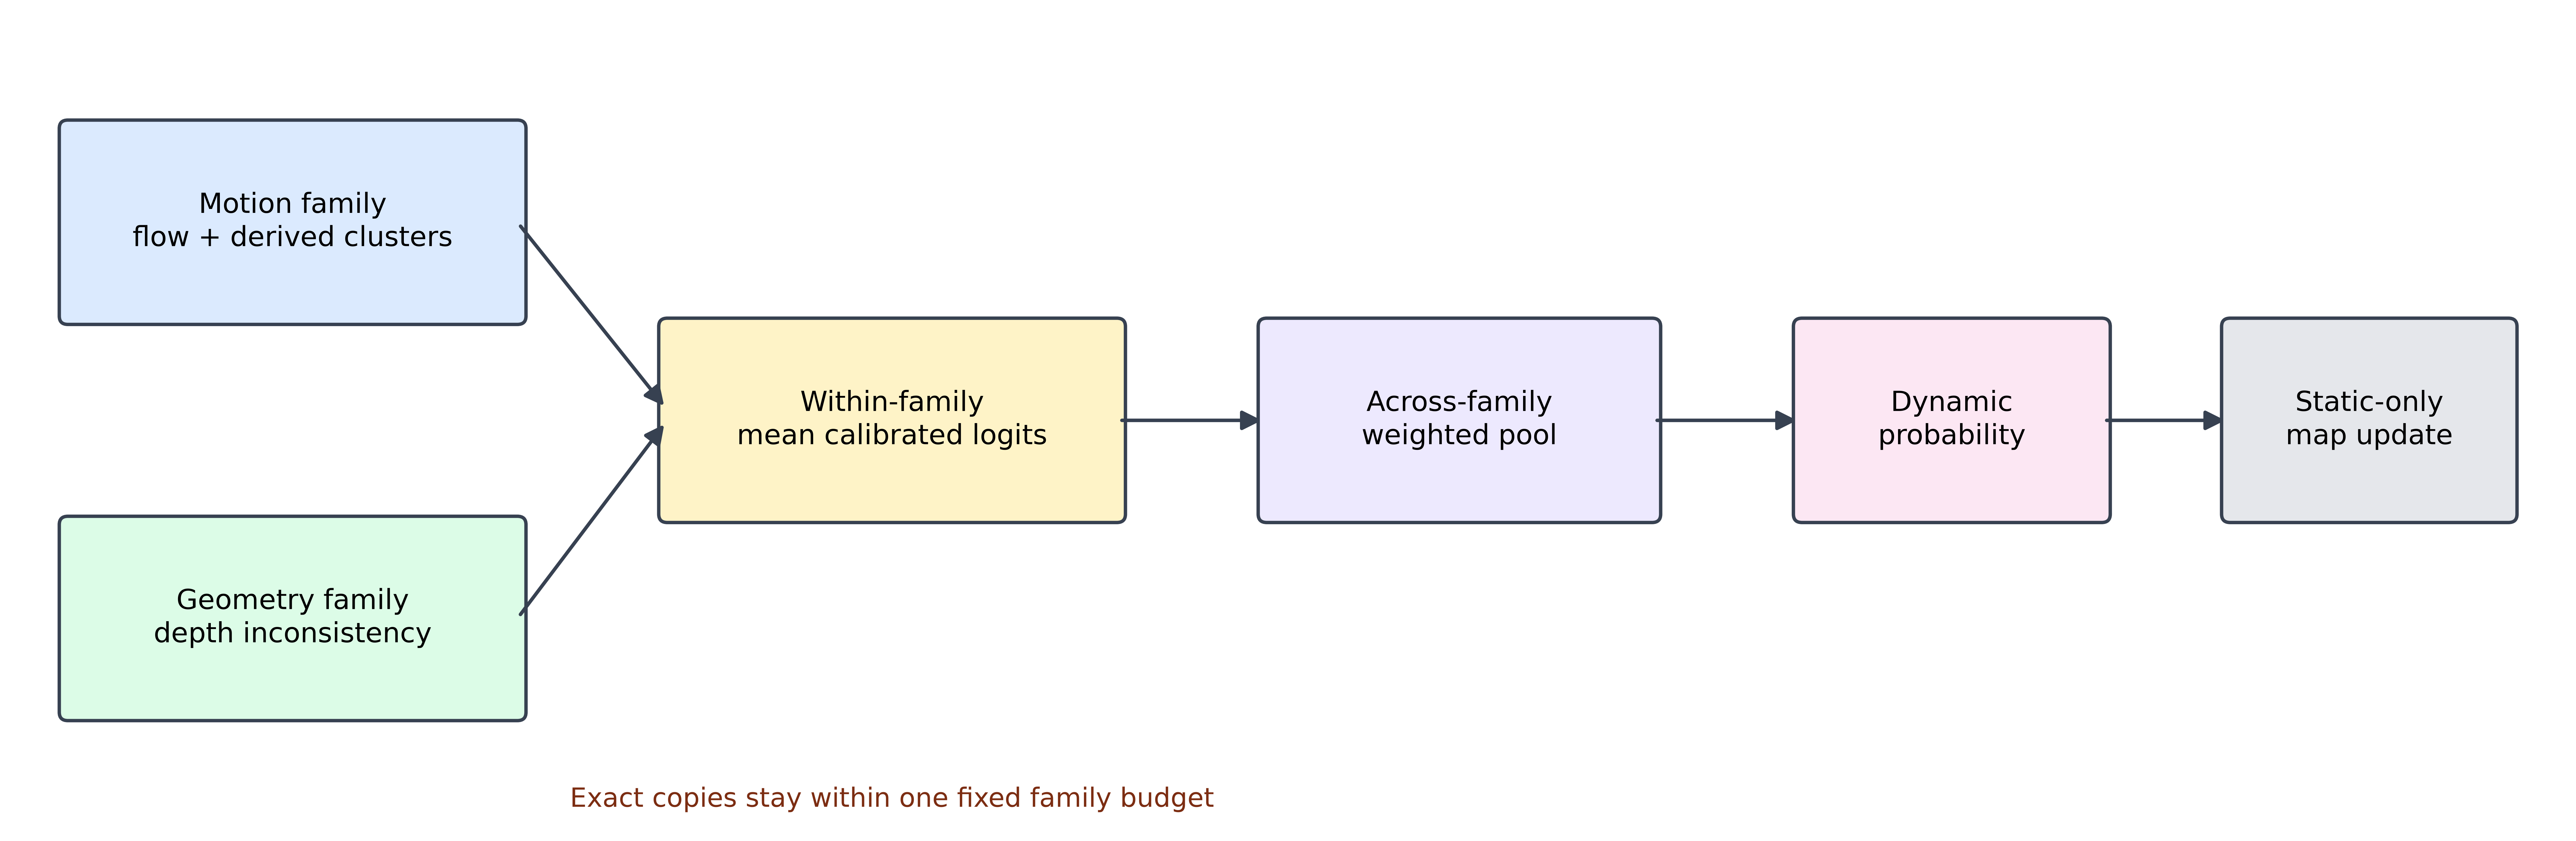
\includegraphics[width=0.96\textwidth]{method_overview.png}
\caption{Source-aware pooling and its connection to mapping. Derived motion cues share one family budget; geometry receives a separate budget. The stress test validates replication behavior, while the mapping experiment validates static-only updates under oracle masks. It does not validate a learned mask front end.}
\label{fig:overview}
\end{figure*}

\subsection{Why a channel product is fragile}
For calibrated probabilities $p_j$, a commonly used heuristic adds logits or multiplies odds:
\begin{equation}
q_{\mathrm{prod}}(D=1\mid x)=\sigmoid\!\left(b+\sum_{j=1}^{J}w_j\logit p_j\right).
\label{eq:prod}
\end{equation}
If the channels were conditionally independent likelihood factors with correct prior handling, a related expression could be justified. Derived vision cues generally do not satisfy that premise. If one channel is copied $K$ times, Eq.~\eqref{eq:prod} changes its contribution from $w\ell$ to $Kw\ell$ although the observation contains no new information. The output moves toward a hard decision as $K$ grows.

Channel averaging avoids unbounded logit growth but creates a different dependence on representation. Adding more motion-derived channels changes the relative weight between motion and geometry. A fixed family budget is intended to preserve the declared balance among sources.

\subsection{Scope of the evidence}
The manuscript answers two mechanism questions:
\begin{enumerate}
\item Does a pooling rule change confidence when an existing derived channel is replicated exactly?
\item Under oracle masks, do initialization filtering and loss masking have distinguishable effects on a Gaussian map?
\end{enumerate}
It does not answer whether a particular real-image flow/depth/cluster pipeline predicts superior masks, whether tracking improves, or whether metric scale is recovered. This boundary determines the title, contribution language, experiments, and comparison policy.

\section{Source-Aware Evidence Pooling}
\subsection{Calibration}
Let a raw channel score be $s_j$. We fit a temperature $T_j>0$ and optional bias $a_j$ on calibration data:
\begin{equation}
p_j(D=1\mid x)=\sigmoid\left(\frac{s_j(x)}{T_j}+a_j\right).
\label{eq:temp}
\end{equation}
Calibration data must be disjoint from the final evaluation set. When scenes are temporally correlated, frame-level random splitting is insufficient; whole sequences or environments should be held out. The synthetic stress test uses independently sampled calibration and test sets to isolate the pooling behavior.

\subsection{Within-family and across-family pooling}
Let $\mathcal S_g=\{j:g(j)=g\}$ contain the channels in family $g$. Define the family logit
\begin{equation}
L_g(x)=\frac{1}{|\mathcal S_g|}\sum_{j\in\mathcal S_g}\logit p_j(D=1\mid x).
\label{eq:familylogit}
\end{equation}
The final probability is
\begin{equation}
\begin{aligned}
q(D=1\mid x)&=\sigmoid\left(b+\sum_{g=1}^{G}\alpha_g L_g(x)\right),\\
\alpha_g&\ge 0,\qquad \sum_g\alpha_g=1.
\end{aligned}
\label{eq:pool}
\end{equation}
Uniform $\alpha_g=1/G$ is the conservative default used in the stress test. Learned weights require nested validation or cross-validation; fitting them on the test set would invalidate the calibration result. The bias $b$ can encode a deployment prior only when that prior is known or estimated without test leakage.

\subsection{Replication invariance}
\textbf{Proposition 1.} If every channel in a family is replaced by $K$ exact copies of itself and all copies remain in the same family, then the pooled probability in Eq.~\eqref{eq:pool} is unchanged.

\textit{Proof.} Let the original family contain logits $\ell_1,\ldots,\ell_m$. Replication produces $K$ copies of each logit. The new family average is
\begin{equation}
\frac{1}{Km}\sum_{i=1}^{m}\sum_{k=1}^{K}\ell_i
=\frac{K}{Km}\sum_{i=1}^{m}\ell_i
=\frac{1}{m}\sum_{i=1}^{m}\ell_i.
\end{equation}
All other family logits and weights are unchanged, so the argument of the sigmoid and the final probability are unchanged. $\square$

This proposition is deliberately modest. It covers exact replication, a necessary sanity check for a provenance-aware rule. It does not prove optimality under partial correlation, miscalibration, label shift, or adversarially wrong families.

\subsection{Non-identical correlated channels}
For two correlated logits $\ell_1$ and $\ell_2$ in a family, averaging reduces the effect of representing both, but it does not estimate their covariance. A statistically efficient model could learn a joint likelihood or a covariance-aware generalized linear model. Such models require more validation data and can overfit scene-specific correlations. Family averaging trades statistical efficiency under a correct joint model for a transparent invariance property and a lower-capacity parameterization.

The rule also assumes that family membership is known. If a geometry channel is derived using motion warping, placing it in a separate family may still double count information. A practical implementation should record a provenance directed acyclic graph, then merge families whenever one branch deterministically contains another. Sensitivity to alternative family assignments belongs in the full real-image study.

\subsection{Missing evidence and numerical safeguards}
If family $g$ is unavailable for a pixel, we renormalize weights over the available set $\mathcal A(x)$:
\begin{equation}
q=\sigmoid\left(b+\sum_{g\in\mathcal A(x)}
\frac{\alpha_g}{\sum_{h\in\mathcal A(x)}\alpha_h}L_g\right).
\label{eq:missing}
\end{equation}
Probabilities are clipped to $[\epsilon,1-\epsilon]$ before taking logits. This is a numerical guard, not a substitute for calibration. Invalid flow, depth discontinuities, occlusions, and saturated semantic scores should be accompanied by validity masks so that missing evidence is not silently treated as strong static evidence.

\section{Dynamic-Aware Gaussian Mapping}
\subsection{Gaussian scene representation}
A Gaussian primitive $i$ has center $\mu_i\in\R^3$, covariance $\Sigma_i$, opacity $o_i$, and color parameters $c_i$. Following 3DGS \cite{kerbl2023}, the covariance is parameterized with a scale and rotation to preserve positive semidefiniteness. Projection through a known camera yields a 2-D footprint. Front-to-back alpha compositing produces a rendered color
\begin{equation}
\hat I_\theta(p)=\sum_{i\in\mathcal N(p)}T_i(p)\,\alpha_i(p)\,c_i,
\quad
T_i(p)=\prod_{k<i}\bigl(1-\alpha_k(p)\bigr),
\label{eq:render}
\end{equation}
where $\theta$ collects Gaussian parameters and $\mathcal N(p)$ is the depth-sorted set contributing to pixel $p$.

The controlled implementation fixes the number of primitives at 2,500 and optimizes their parameters for 1,200 iterations. It does not implement the complete densification, pruning, tracking, loop closure, or keyframe logic required by a production SLAM system. This simplification is intentional: it keeps the intervention on dynamic pixels observable.

\subsection{Two intervention points}
Dynamic suppression can act before or during optimization. Initialization filtering back-projects only pixels labeled static. This prevents a moving object from directly creating initial Gaussians. However, those Gaussians are subsequently optimized against all training frames unless the objective is also masked. Static primitives can then change color, opacity, scale, or position to explain a transient.

Given a dynamic probability $q_t(p)$ for frame $t$, define static weight $w_t(p)=1-q_t(p)$. The masked photometric term is
\begin{equation}
\mathcal L_{\mathrm{photo}}=
\frac{\sum_{t,p}w_t(p)\left\lVert \hat I_{\theta,t}(p)-I_t(p)\right\rVert_1}
{3\sum_{t,p}w_t(p)+\epsilon}.
\label{eq:masked}
\end{equation}
The denominator normalizes for the number of valid color channels. A full implementation can mix L1 with structural similarity as in 3DGS. Our reported training intervention uses the saved experimental implementation; the held-out evaluation reports both PSNR and its inherited box-window SSIM, explicitly without claiming cross-paper metric identity.

\subsection{Soft versus hard masks}
The family pool yields a soft probability, while the mapping study uses oracle binary masks to isolate optimization. Soft masks preserve uncertain pixels with reduced weight and keep the objective differentiable with respect to upstream parameters. Hard masks prevent ambiguous high-residual pixels from dominating but can remove genuinely static structure. A complete system must compare both and report threshold selection on validation data. The present results establish only that masking matters when the mask is correct.

\subsection{Coordinate and scale conventions}
Camera-to-world and world-to-camera transforms must not be interchanged. Depth back-projection assumes metric or consistently scaled depth and a declared camera model. In a monocular system, a learned metric-depth prior can inject scale, whereas pure projective reconstruction is defined only up to similarity. Therefore, ATE values must state whether trajectories are aligned by $SE(3)$ or $Sim(3)$. Our known-pose experiment uses one fixed synthetic coordinate system and does not evaluate scale observability.

\section{Experimental Protocol}\label{sec:required}
\subsection{Research questions}
The evaluation is organized around four questions:
\begin{description}
\item[RQ1:] Does exact replication degrade probabilistic quality for a fixed channel product?
\item[RQ2:] Is the source-family pool exactly invariant in the implemented stress test?
\item[RQ3:] In known-pose mapping, what is gained by static-only initialization?
\item[RQ4:] Does masking the optimization loss add a consistent gain beyond initialization filtering?
\end{description}

No research question concerns trajectory accuracy or real-mask prediction, so those quantities are not reported as results.

\subsection{Evidence-replication stress test}
For each of ten seeds, a latent log-odds variable generates a binary label. Noisy motion and geometry observations are conditionally related through that latent variable. A temperature is estimated from 10,000 calibration samples, and 50,000 independently sampled test cases are evaluated. The same motion observation is represented one, two, four, or eight times.

We compare three rules. \textit{Fixed product} adds one geometry logit and every represented motion logit. \textit{Channel mean} averages all represented channel logits. \textit{Family pool} first averages the motion family and then gives motion and geometry equal family budgets. Because the replicated motion values are exact copies, a robust provenance rule should not change.

NLL and Brier score are proper scoring rules. Ten-bin ECE summarizes the gap between confidence and accuracy, with the usual dependence on binning. F1 applies a threshold and measures discrimination at that operating point; it is not a calibration metric. We report mean and sample standard deviation over seeds.

\subsection{Known-pose synthetic mapping}
The scene contains simple static geometry and one moving object. Twelve RGB frames are rendered at $160\times120$ pixels. Ground-truth depths and camera poses are available. Training views are $\{0,1,3,4,6,7,9,10\}$; held-out views are $\{2,5,8,11\}$. The split is fixed before optimization.

Three configurations isolate the controls:
\begin{enumerate}
\item \textbf{All pixels}: all observations can initialize Gaussians and contribute to the loss.
\item \textbf{Static initialization}: oracle dynamic pixels do not seed Gaussians, but all pixels contribute to optimization.
\item \textbf{Static initialization plus masked loss}: oracle dynamic pixels are excluded from both initialization and the loss.
\end{enumerate}
Each configuration runs for seeds 0, 1, and 2 with 2,500 Gaussians and 1,200 iterations. The hardware is an NVIDIA GeForce RTX 5060 Ti; the recorded software environment is Python 3.12.3, PyTorch 2.11.0+cu128, and CUDA 12.8.

\subsection{Metrics}
Static-region PSNR is computed on held-out pixels labeled static. The dynamic ghost residual is the mean absolute difference between the Gaussian render and the static clean background inside the region occupied by the moving object. A lower value indicates that less transient appearance remains in the persistent map. We additionally record whole-image PSNR, clean-background PSNR, box-window SSIM, wall-clock optimization time, render time, and peak allocated GPU memory.

The full-image PSNR can fall when the target image includes the moving object but the desired persistent map does not. It is therefore not the primary metric for a static-map objective. Static-region PSNR and ghost residual directly address the intended result. This metric choice is specified before interpreting the runs.

\subsection{Statistical reporting}
With three mapping seeds, asymptotic significance tests would be fragile and easy to overinterpret. We report the individual values, mean, sample standard deviation, and paired differences. Consistency of sign across all three seeds is treated as descriptive evidence, not a population-level guarantee. The fusion study has ten seeds and is likewise summarized without claiming that synthetic sampling captures all real-image correlations.

\section{Results}
\subsection{Replication stress test}
Fig.~\ref{fig:fusion} reports all four metrics. With one motion channel, the three rules coincide at NLL $0.4788\pm0.0023$, Brier $0.1578\pm0.0009$, ECE $0.0148\pm0.0019$, and F1 $0.6388\pm0.0039$. This equality is an important control: the methods differ only after representation changes.

\begin{figure*}[t]
\centering
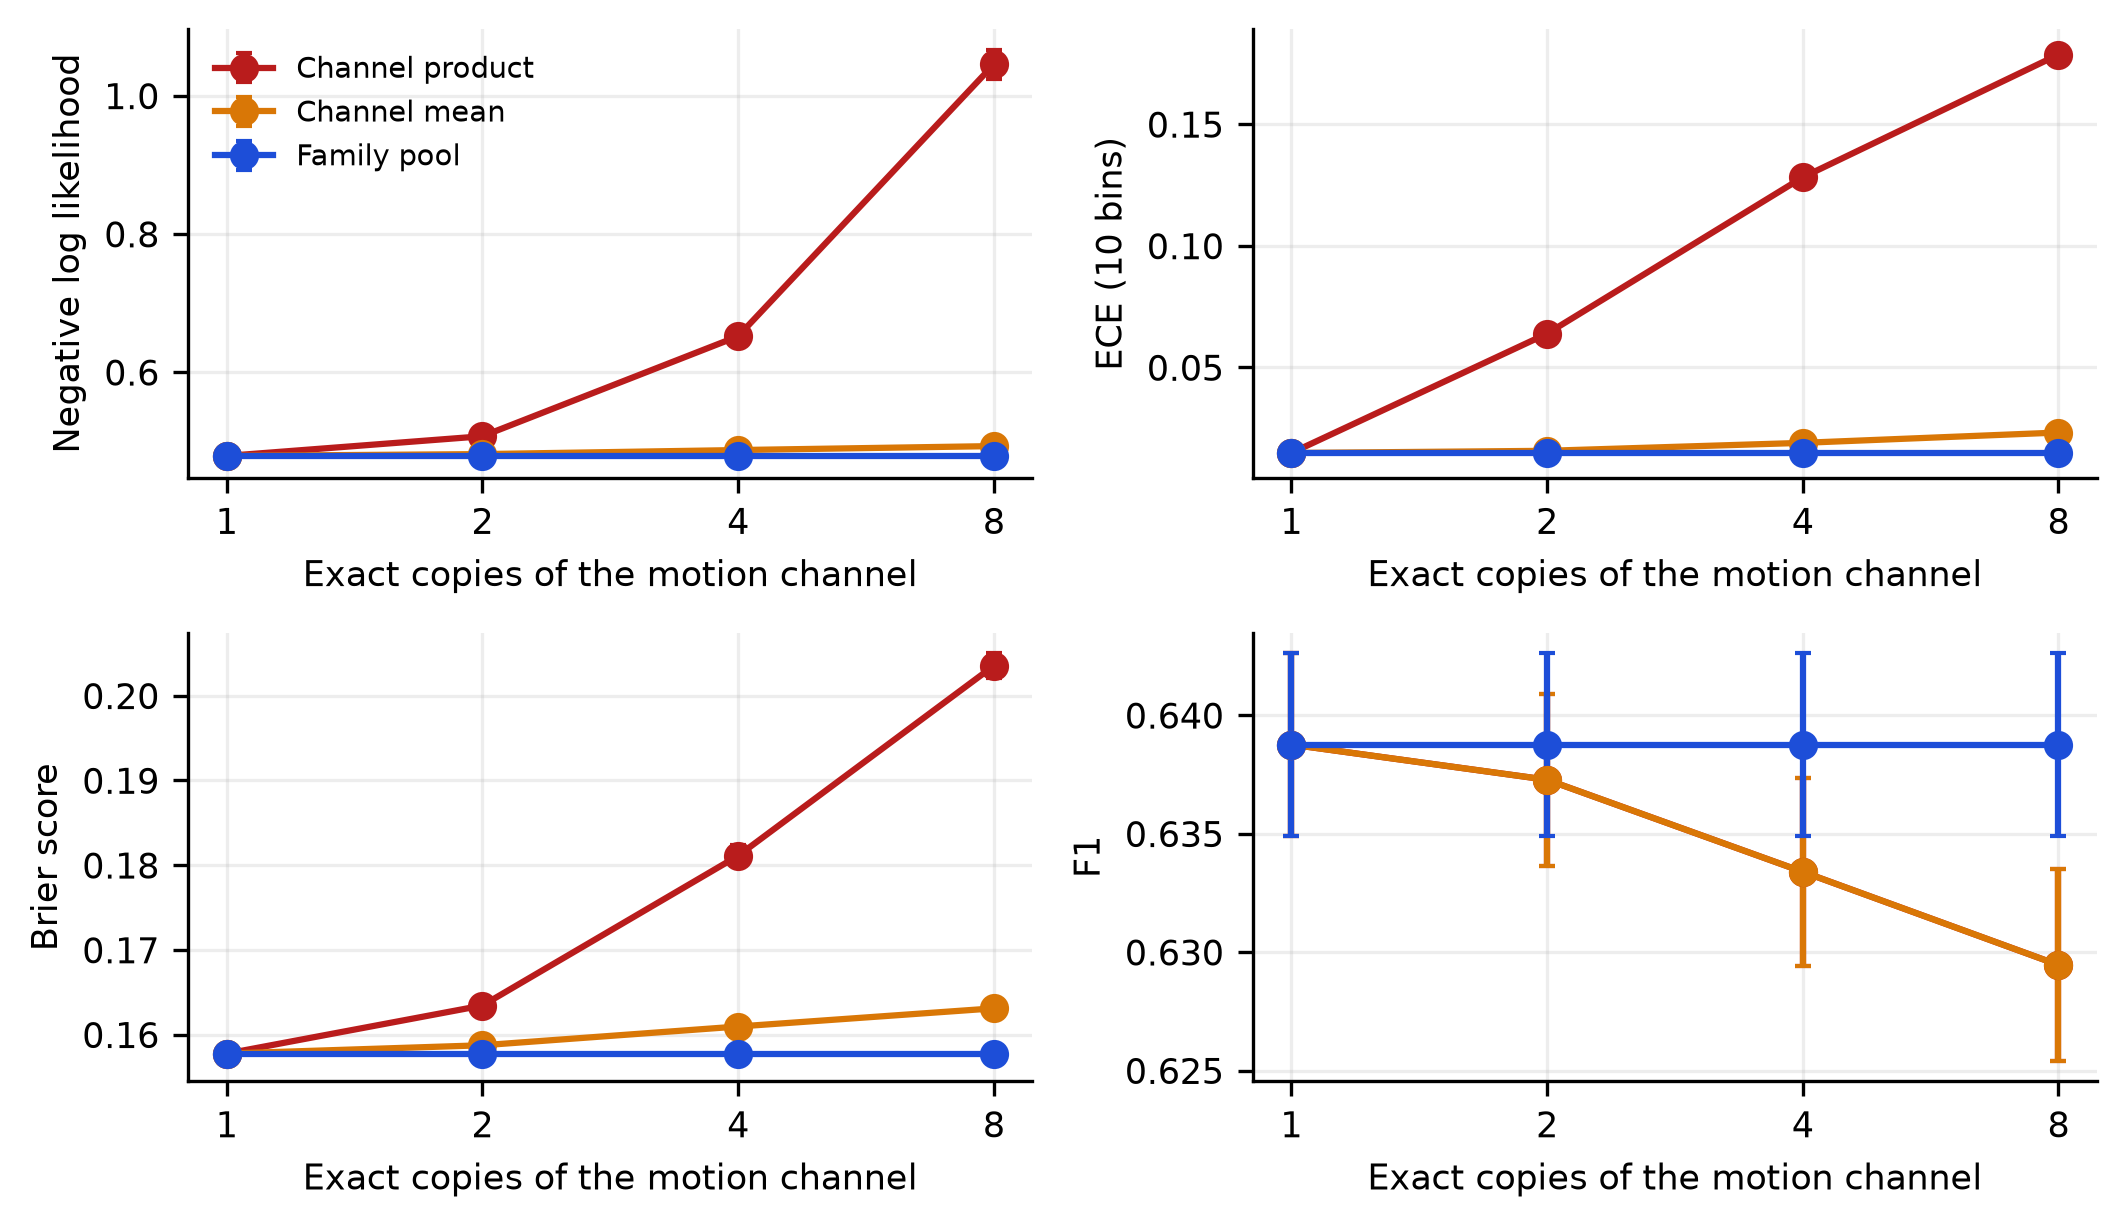
\includegraphics[width=0.92\textwidth]{fusion_stress_extended.png}
\caption{Exact-replication stress test over ten seeds. Error bars are sample standard deviations. The fixed channel product becomes sharply overconfident as one motion observation is copied. Channel averaging limits the damage but changes the motion/geometry balance. The source-family pool is invariant by construction.}
\label{fig:fusion}
\end{figure*}

At eight copies, fixed-product NLL rises to $1.0455\pm0.0210$, Brier score to $0.2035\pm0.0015$, and ECE to $0.1787\pm0.0020$. The F1 score changes only from $0.6388$ to $0.6295$, illustrating why thresholded discrimination alone can hide a severe confidence defect. Channel averaging is substantially more stable than the product but is not invariant: at eight copies its NLL is $0.4930\pm0.0023$ and ECE is $0.0232\pm0.0031$.

The family pool remains numerically identical at every replication level: NLL $0.4788\pm0.0023$, Brier $0.1578\pm0.0009$, ECE $0.0148\pm0.0019$, and F1 $0.6388\pm0.0039$. This answers RQ1 and RQ2 for the implemented sanity test. It does not show that family pooling is best when genuinely new, partly correlated channels are added.

\begin{table}[t]
\caption{Fusion results at one and eight motion copies. Mean $\pm$ sample SD over ten seeds.}
\label{tab:fusion}
\centering\scriptsize
\begin{tabular}{llcc}
\toprule
Copies & Method & NLL & ECE$_{10}$ \\
\midrule
1 & Fixed product & $0.4788\pm0.0023$ & $0.0148\pm0.0019$ \\
1 & Channel mean & $0.4788\pm0.0023$ & $0.0148\pm0.0019$ \\
1 & Family pool & $0.4788\pm0.0023$ & $0.0148\pm0.0019$ \\
\midrule
8 & Fixed product & $1.0455\pm0.0210$ & $0.1787\pm0.0020$ \\
8 & Channel mean & $0.4930\pm0.0023$ & $0.0232\pm0.0031$ \\
8 & Family pool & $0.4788\pm0.0023$ & $0.0148\pm0.0019$ \\
\bottomrule
\end{tabular}
\end{table}

\subsection{Aggregate mapping results}
Table~\ref{tab:mapping} and Fig.~\ref{fig:mapping} summarize the held-out mapping runs. Static-only initialization improves static-region PSNR from $27.671\pm0.517$ to $29.459\pm0.436$~dB. Adding the masked loss raises it further to $31.705\pm0.228$~dB. The complete intervention improves PSNR by $4.034\pm0.733$~dB relative to all-pixel training; the 5 paired improvements are 3.186, 3.927, 4.132, 5.183, 3.740~dB.

\begin{figure*}[t]
\centering
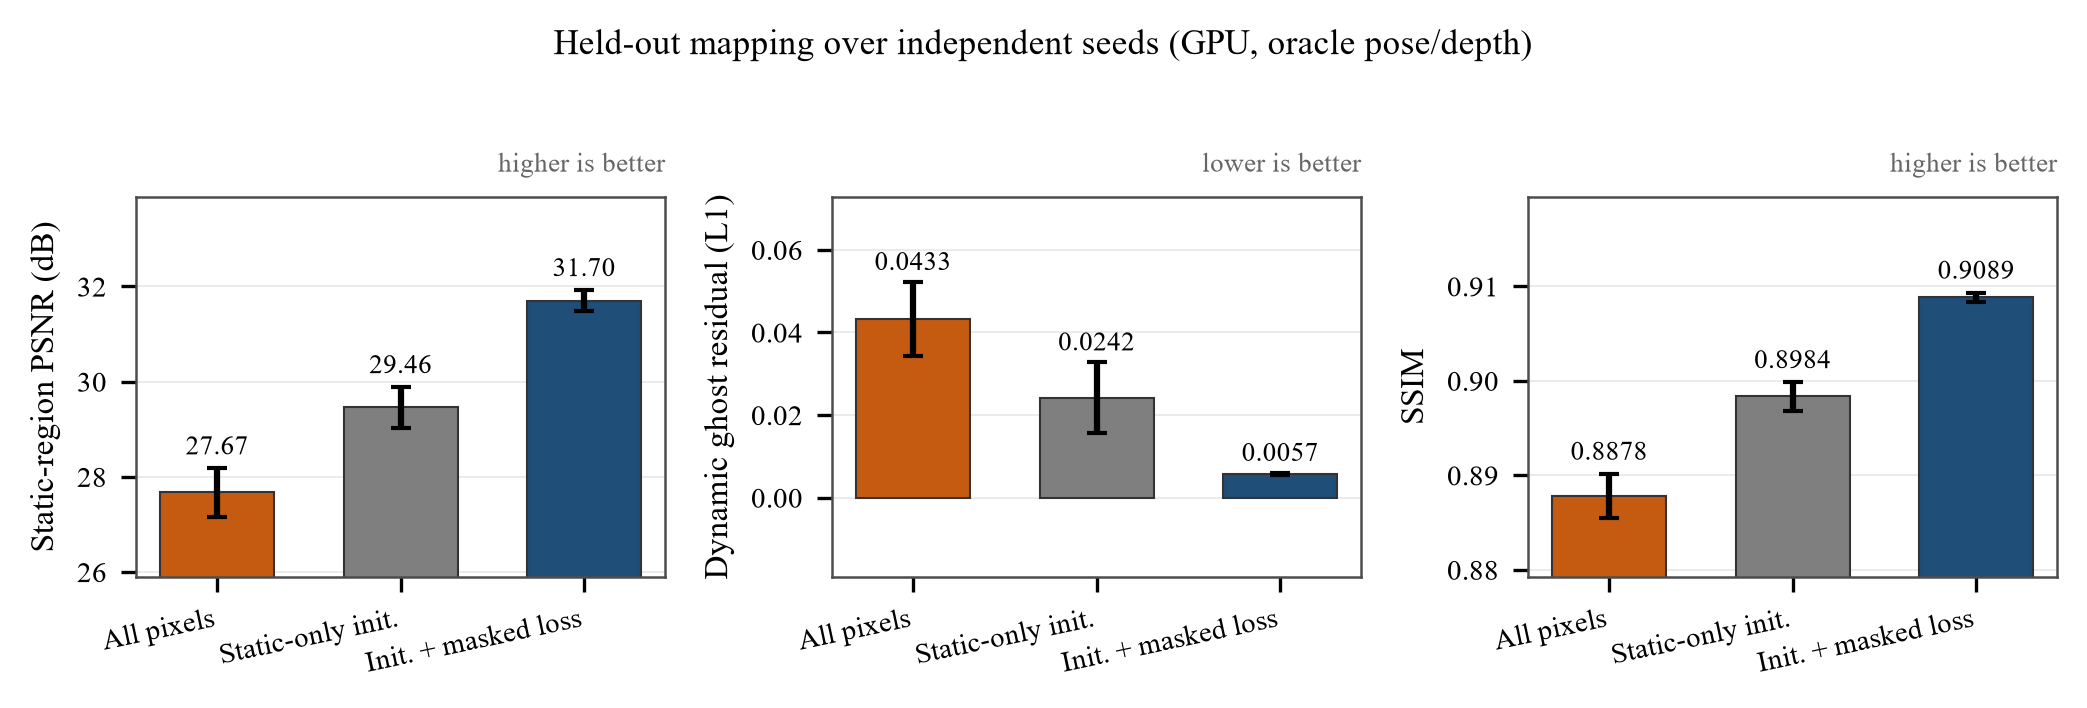
\includegraphics[width=0.94\textwidth]{mapping_summary.png}
\caption{Held-out mapping summary over 5 seeds. Error bars are sample standard deviations. Static-only initialization helps, but loss masking supplies the larger and more stable reduction in transient contamination.}
\label{fig:mapping}
\end{figure*}

\begin{table}[t]
\caption{Held-out mapping results. Mean ± sample SD over 5 seeds.}
\label{tab:mapping}
\centering\scriptsize
\begin{tabular}{lccc}
\toprule
Configuration & Static PSNR & Ghost L1 & SSIM \\
\midrule
All pixels & 27.671$\pm$0.517 & 0.0433$\pm$0.0089 & 0.8878$\pm$0.0024 \\
Static init. & 29.459$\pm$0.436 & 0.0242$\pm$0.0086 & 0.8984$\pm$0.0015 \\
Init. + mask & 31.705$\pm$0.228 & 0.0057$\pm$0.0002 & 0.9089$\pm$0.0005 \\
\bottomrule
\end{tabular}
\end{table}

In the matched three-seed subset, ghost residual falls from $0.0383\pm0.0045$ to $0.0270\pm0.0103$ after initialization filtering, but this intermediate result is variable: seed 0 has residual 0.0359, close to the all-pixel value. After loss masking, the residual is $0.0058\pm0.0003$. The paired reduction is $0.0325\pm0.0047$, or a $6.64\pm0.99$-fold ratio. All seeds agree on the direction of the complete intervention. These results answer RQ3 and RQ4 within the oracle, known-pose setting.

\subsection{Per-seed consistency}

Fig.~\ref{fig:seedvar} opens the aggregate numbers into per-seed pairs. The masked configuration is the best of the three for every seed, and the gap is larger than the seed-to-seed spread within any single configuration. The intermediate static-initialization configuration is the most variable one: its advantage over all-pixel training depends on whether the retained primitives happen to cover the transient object.

\begin{figure*}[t]
\centering
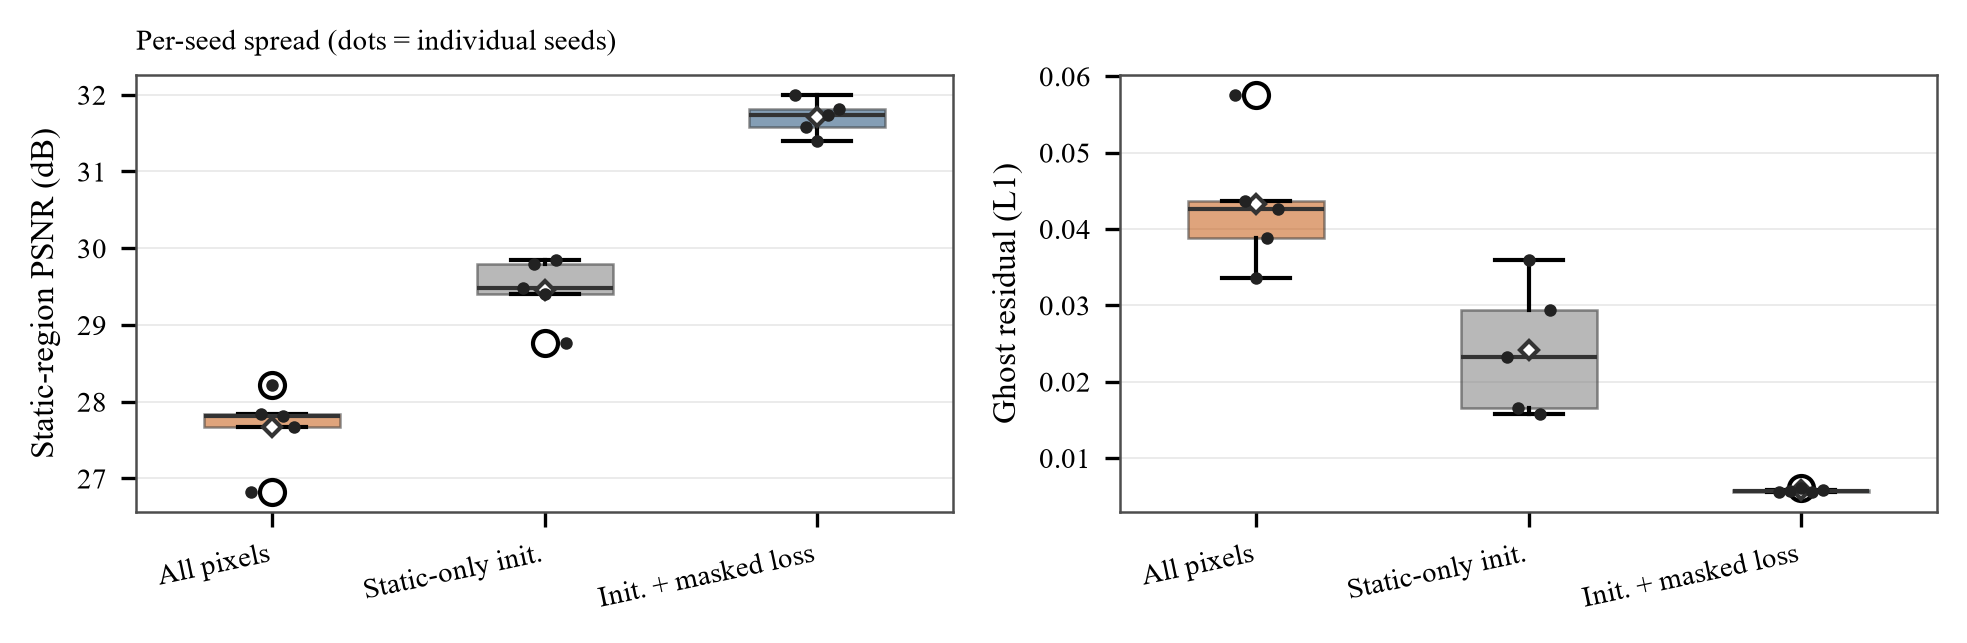
\includegraphics[width=0.78\textwidth]{seed_variance.png}
\caption{Per-seed paired results for the three training configurations. Each marker is one independent GPU run on the same held-out views; lines connect configurations that share a seed. The ordering is preserved for every seed, so the aggregate improvement is not produced by a lucky initialization.}
\label{fig:seedvar}
\end{figure*}


\subsection{Per-view behavior}
Fig.~\ref{fig:perview} shows that the aggregate result is not driven by one view. The full configuration has the highest static-region PSNR for views 2, 5, 8 and 11. Its mean per-view PSNR values are 29.468, 30.008, 33.711, 33.633~dB. The corresponding all-pixel means are 27.092, 27.119, 31.480, 24.994~dB.

\begin{figure*}[t]
\centering
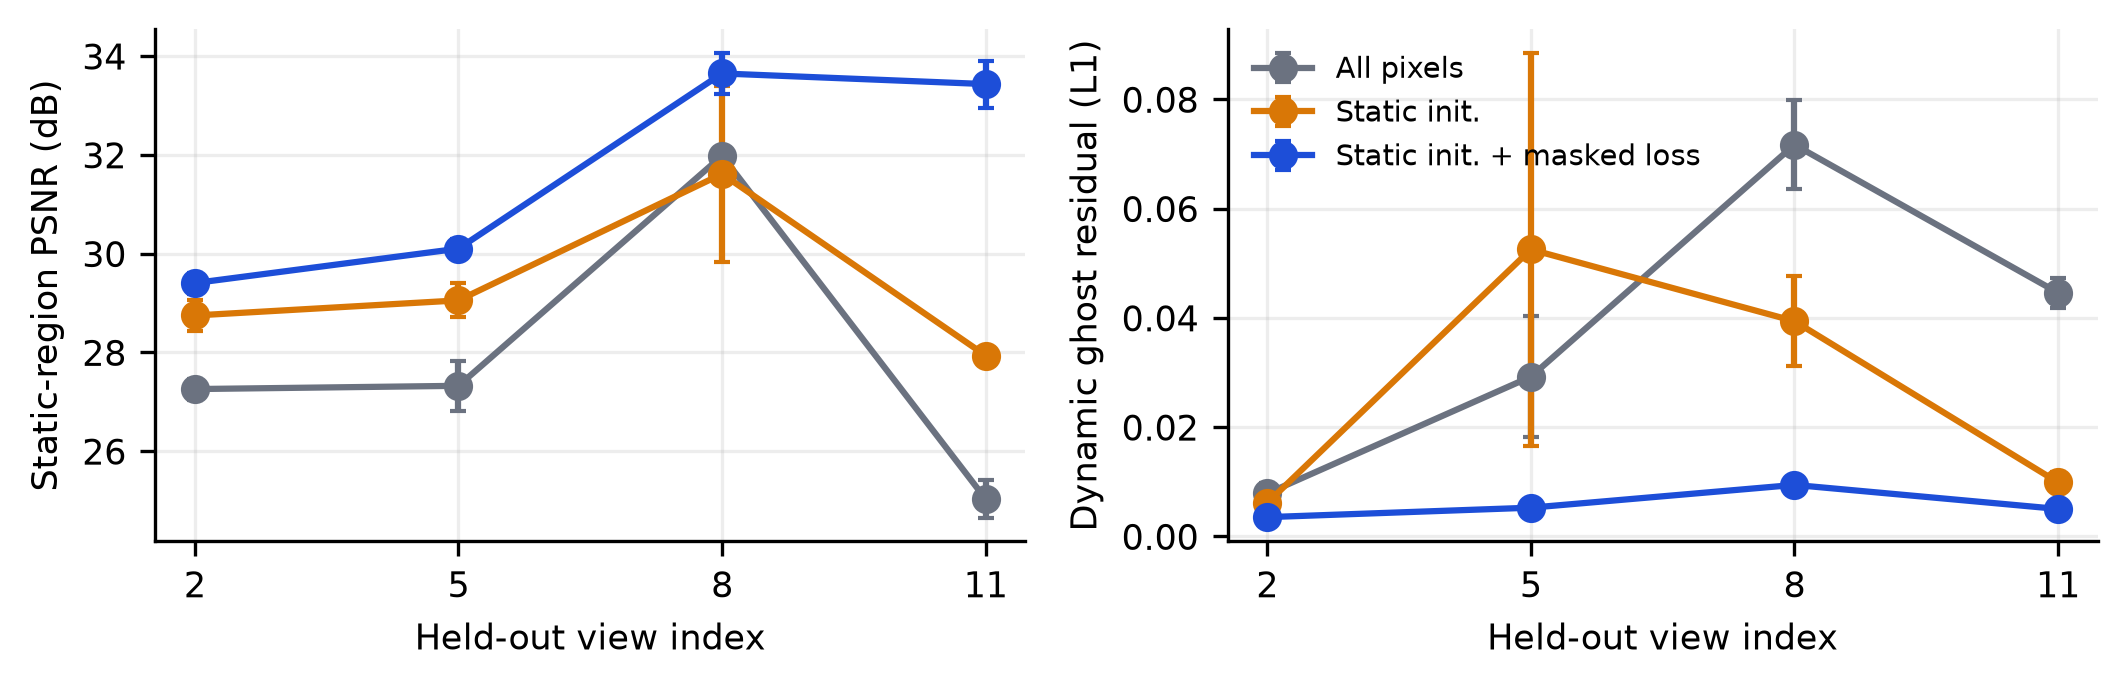
\includegraphics[width=0.92\textwidth]{per_view_results.png}
\caption{Per-view held-out results averaged over 5 seeds. Loss masking is especially important for views 8 and 11, where the all-pixel map leaves larger transient residuals.}
\label{fig:perview}
\end{figure*}

The ghost-residual profile explains why initialization alone is insufficient. On view 5, static-only initialization has residual $0.0525\pm0.0360$, worse than the all-pixel mean $0.0292\pm0.0111$. This does not imply that initialization filtering is harmful in general; it shows that unmasked optimization can still bend the remaining Gaussians toward transient pixels. The full configuration reduces the view-5 residual to $0.0053\pm0.0004$ and keeps every view at or below 0.0094.

\subsection{Qualitative comparison}
Fig.~\ref{fig:qual} shows held-out view 8 for seed 0. All-pixel optimization leaves a visible orange/green trace in the rendered region where the moving sphere appears in the observation. Static-only initialization weakens but does not remove the artifact. The masked-loss configuration renders the static background more cleanly. The figure is a visualization of the saved run, not a cherry-picked claim of natural-image quality; the scene is intentionally simple and the displayed frame is one of four declared held-out views.

Fig.~\ref{fig:qualgrid} extends the single-view comparison to all four held-out views. The same ordering holds across the grid: all-pixel training leaves transient structure, static-only initialization weakens it unevenly, and the masked configuration removes it. Because the tiles are upsampled with nearest-neighbour interpolation, the displayed pixels are exactly the rendered pixels; no smoothing was applied to make the comparison look cleaner.

\begin{figure*}[t]
\centering
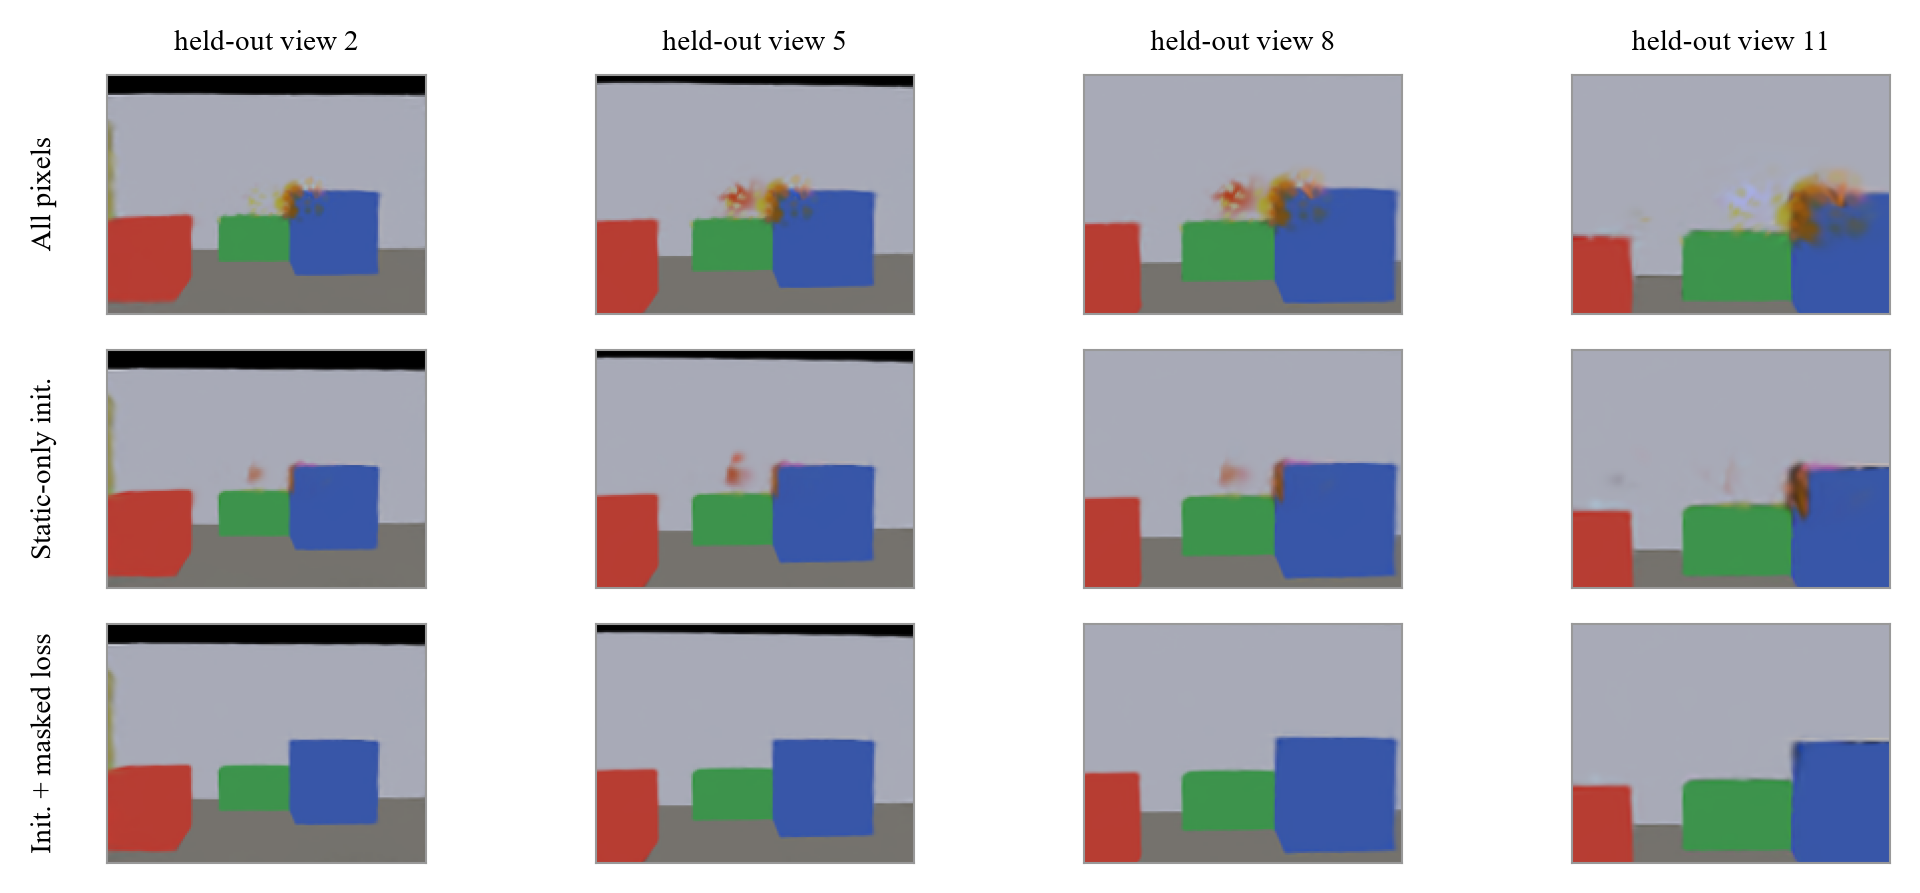
\includegraphics[width=0.95\textwidth]{qualitative_grid.png}
\caption{Full qualitative grid: three training configurations (rows) against the four declared held-out views (columns). Each tile shows the optimized render; the dynamic input and the static reference are shown in Fig.~\ref{fig:qual}. Tiles are enlarged with nearest-neighbour interpolation so that no pixel value is invented by the display.}
\label{fig:qualgrid}
\end{figure*}

Fig.~\ref{fig:failzoom} magnifies the failure region instead of the whole frame. The absolute-error map makes the mechanism visible: all-pixel training paints the transient object into the map, the error concentrates exactly on that region, and the masked configuration reduces it without blurring the surrounding static structure.

\begin{figure*}[t]
\centering
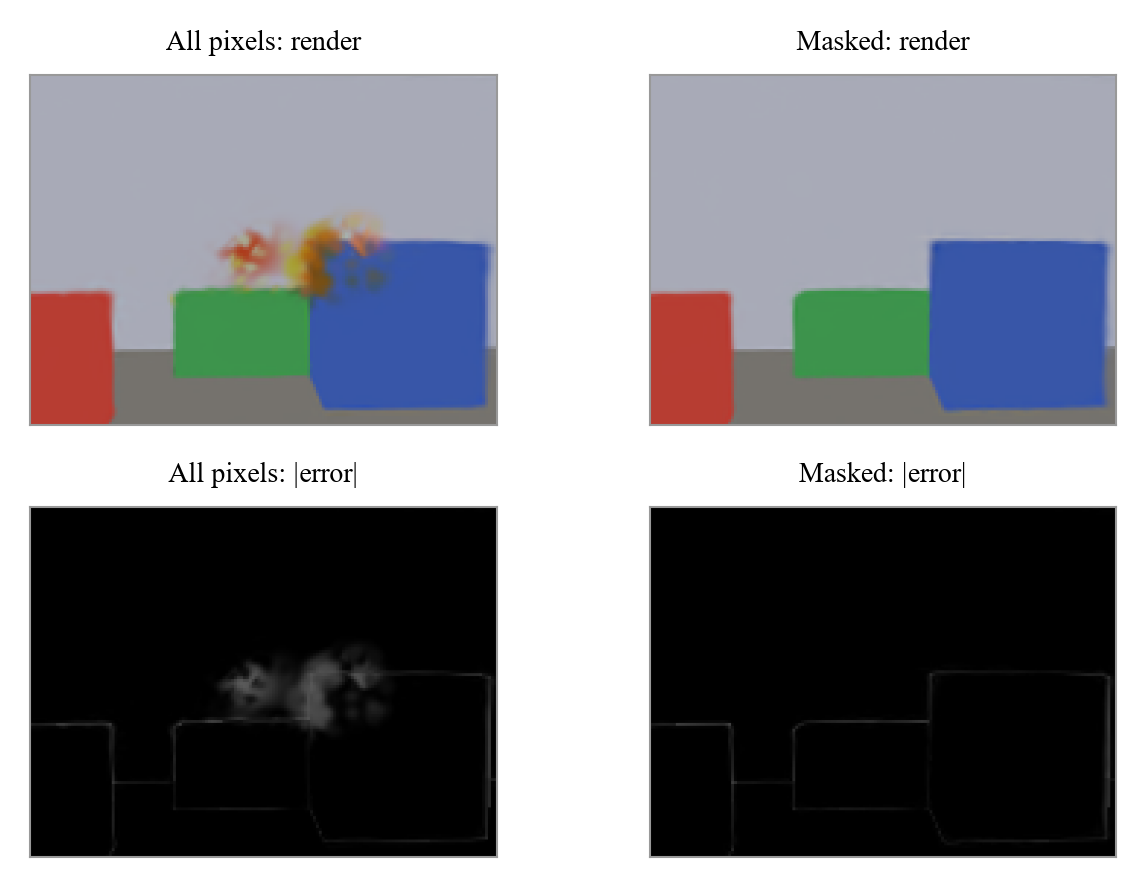
\includegraphics[width=0.55\textwidth]{failure_zoom.png}
\caption{Local $3\times$ magnification of the render and the absolute error map for held-out view 8. The error map is computed against the dynamic-free reference, so bright pixels mark transient content that the persistent map should not contain.}
\label{fig:failzoom}
\end{figure*}


\begin{figure*}[t]
\centering
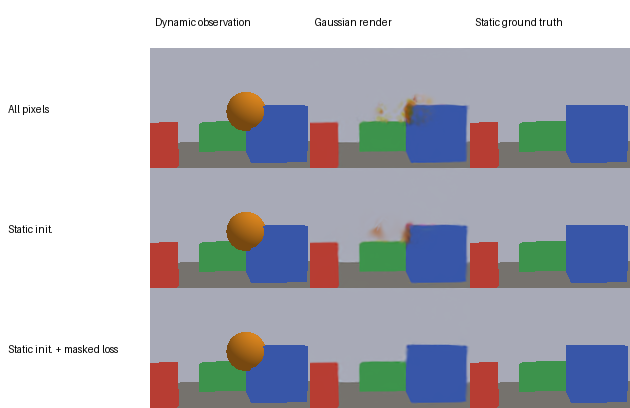
\includegraphics[width=0.86\textwidth]{qualitative_view8.png}
\caption{Qualitative held-out comparison for view 8, seed 0. Columns show the dynamic input, the optimized Gaussian render, and the static ground truth. Rows show the three training configurations.}
\label{fig:qual}
\end{figure*}

\subsection{Resource profile}
Fig.~\ref{fig:resources} reports recorded resource use. Mean optimization time is 112.19 s for all-pixel training and approximately 107.6 s for both static-aware configurations. The all-pixel standard deviation is larger because seed 0 took 121.58 s while the other runs were near 107.49 s. Mean render times are 25.69, 25.72, and 25.74 ms per frame, corresponding to roughly 39 frames/s in this small controlled renderer. Peak allocated GPU memory is approximately 2.94 GiB for every mode.

\begin{figure*}[t]
\centering
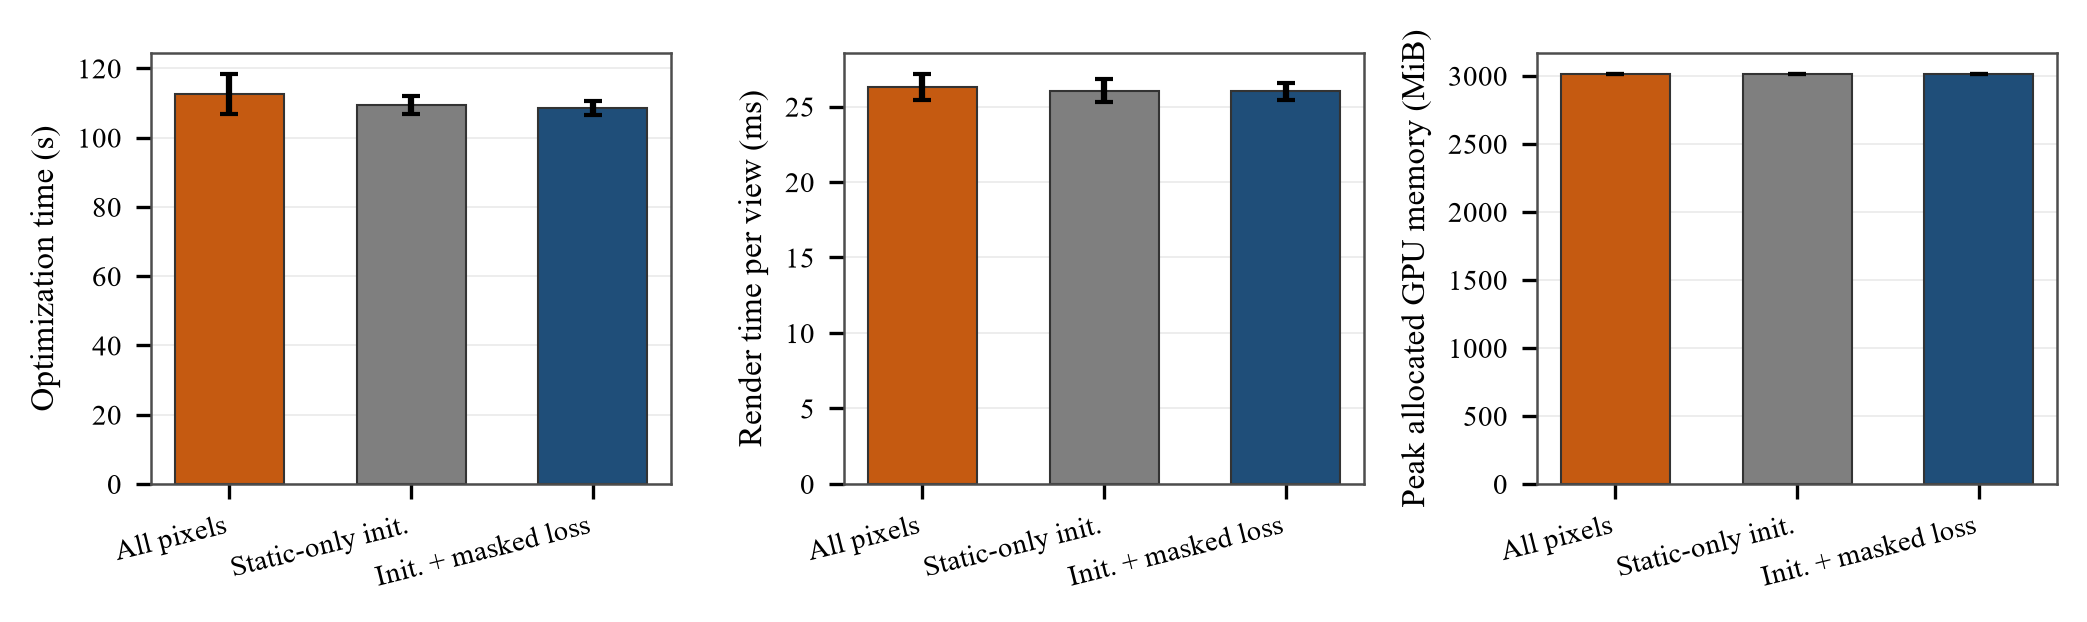
\includegraphics[width=0.93\textwidth]{resource_profile.png}
\caption{Recorded optimization time, render time, and peak allocated GPU memory. These measurements characterize the controlled implementation only and are not a synchronized end-to-end SLAM throughput claim.}
\label{fig:resources}
\end{figure*}

Fig.~\ref{fig:curves} shows where the trajectories separate. The all-pixel objective reaches a lower training loss because it is allowed to explain the moving object, which is precisely why a low photometric loss is not evidence of a clean map. The masked objective settles at a higher loss while producing the better held-out static reconstruction, and this divergence between training loss and held-out static fidelity is the practical reason the protocol holds out views instead of reporting the optimized objective.

\begin{figure*}[t]
\centering
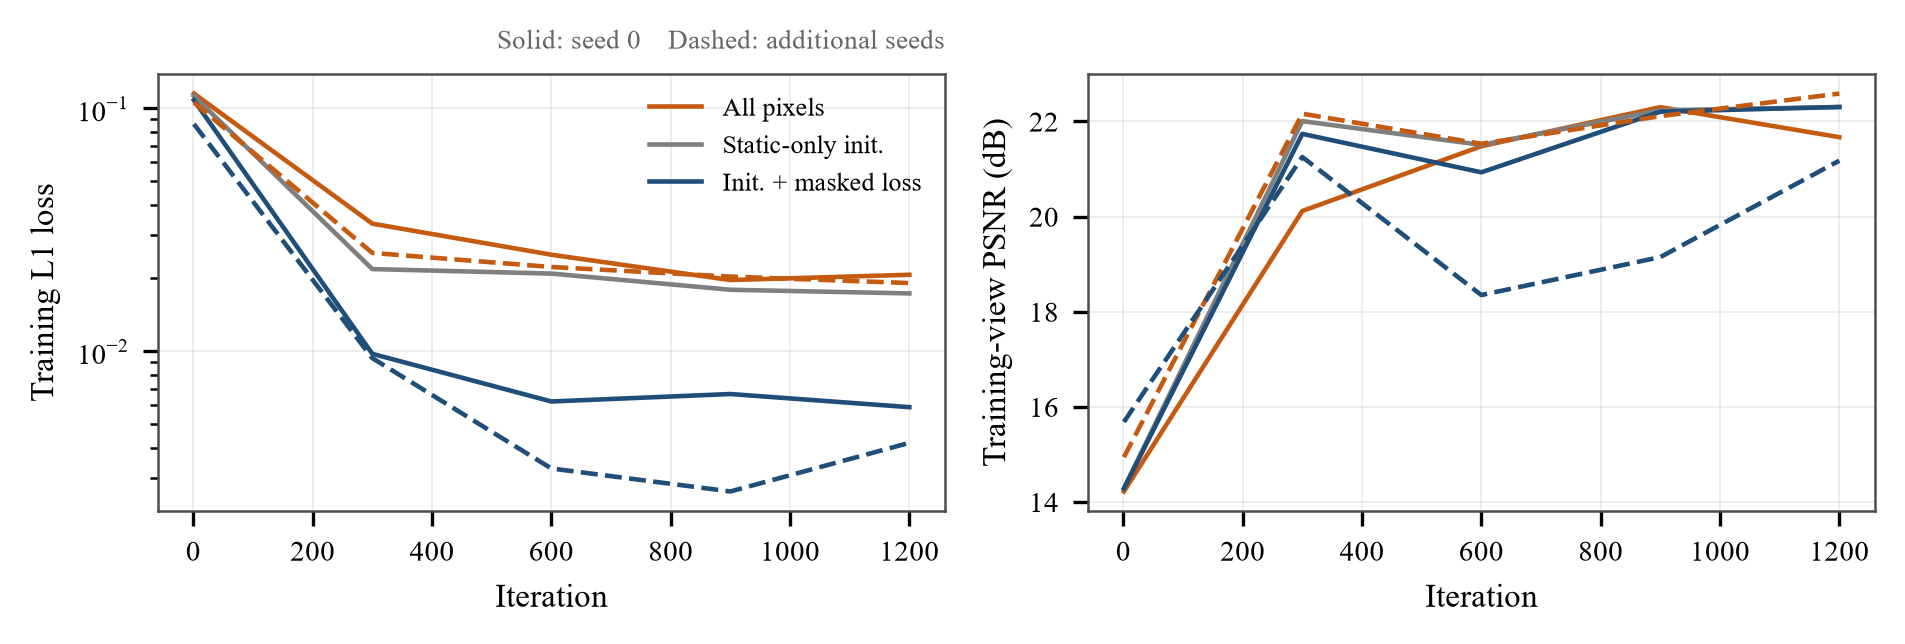
\includegraphics[width=0.94\textwidth]{training_curves.png}
\caption{Optimization histories on a logarithmic loss axis, one panel per configuration, all seeds overlaid. The curves show where the configurations diverge rather than only where they end.}
\label{fig:curves}
\end{figure*}

The similar resource profile is expected because all modes render the same number of Gaussians and differ mainly in data selection and loss weighting. We do not report the inverse render time as ``system FPS'': it excludes image loading, flow/depth inference, mask calibration, tracking, map maintenance, synchronization, and visualization.

\subsection{Capacity, budget, and mask-quality ablations}
A single operating point cannot show whether the mapping conclusion is an artifact of the chosen capacity or schedule. We therefore repeat the masked configuration across three axes, holding the data split, seeds, and metric definitions fixed. Table~\ref{tab:ablation} reports the result; all runs are independent GPU executions with the same protocol as the main experiment.

\textbf{Capacity.} Varying the number of Gaussian primitives from 1{,}000 to 5{,}000 changes static-region PSNR from 30.55 to 31.87~dB. The gain is modest relative to the gap between all-pixel training and the masked configuration, which indicates that the reported improvement is not produced by giving the model more primitives.

\textbf{Optimization budget.} Extending training from 600 to 2{,}400 iterations moves static-region PSNR from 30.62 to 32.38~dB. Only the combined masked configuration was run in this budget sweep. It establishes sensitivity within that configuration; it does not establish a matched-budget gap against the other configurations.

\textbf{Mask-label noise.} Real mask predictors are imperfect, so we perturb the oracle mask by flipping labels at 5\%, 10\%, and 20\% of the pixels. Static-region PSNR changes from 31.70~dB at the clean mask to 31.55~dB at 20\% noise, while the ghost residual moves from 0.0057 to 0.0062. The response is non-monotone and small; this experiment cannot substitute for measuring a real predictor whose errors are spatially correlated.

\textbf{Morphology audit.} The implementation applies max pooling to the static-validity mask. Positive dilation expands static support, equivalently eroding the excluded dynamic region; negative dilation contracts static support. The nominal soft mask equals the hard mask for binary labels and is not treated as a distinct soft-mask experiment.

\begin{table}[t]
\caption{Ablation matrix for the masked configuration. Mean ± sample SD over independent seeds; each row holds the remaining factors fixed.}
\label{tab:ablation}
\centering\scriptsize
\begin{tabular}{llccc}
\toprule
Factor & Setting & Static PSNR & Ghost L1 & Runs \\
\midrule
Gaussians & 1,000 & 30.55$\pm$0.22 & 0.0100$\pm$0.0006 & 2 \\
Gaussians & 5,000 & 31.87$\pm$0.03 & 0.0057$\pm$0.0001 & 2 \\
\midrule
Iterations & 600 & 30.62$\pm$0.08 & 0.0074$\pm$0.0008 & 2 \\
Iterations & 2,400 & 32.38$\pm$0.06 & 0.0057$\pm$0.0003 & 2 \\
\midrule
Mask noise & 0\% (oracle) & 31.70$\pm$0.23 & 0.0057$\pm$0.0002 & 5 \\
Mask noise & 5\% & 31.59$\pm$0.20 & 0.0059$\pm$0.0002 & 2 \\
Mask noise & 10\% & 31.61$\pm$0.16 & 0.0060$\pm$0.0003 & 2 \\
Mask noise & 20\% & 31.55$\pm$0.18 & 0.0062$\pm$0.0004 & 2 \\
\midrule
Morphology & hard oracle (main) & 31.70$\pm$0.23 & 0.0057$\pm$0.0002 & 5 \\
Static support & expanded 2 px & 31.24 & 0.0066 & 1 \\
Static support & contracted 2 px & 31.20 & 0.0065 & 1 \\
\bottomrule
\end{tabular}
\end{table}

Fig.~\ref{fig:ablpts} isolates capacity. Increasing the primitive count from 1{,}000 to 5{,}000 raises static-region PSNR and lowers the ghost residual, but the movement along both axes is small compared with the distance between configurations in Table~\ref{tab:mapping}. The reported advantage of loss masking is therefore not a capacity artefact.

\begin{figure}[t]
\centering
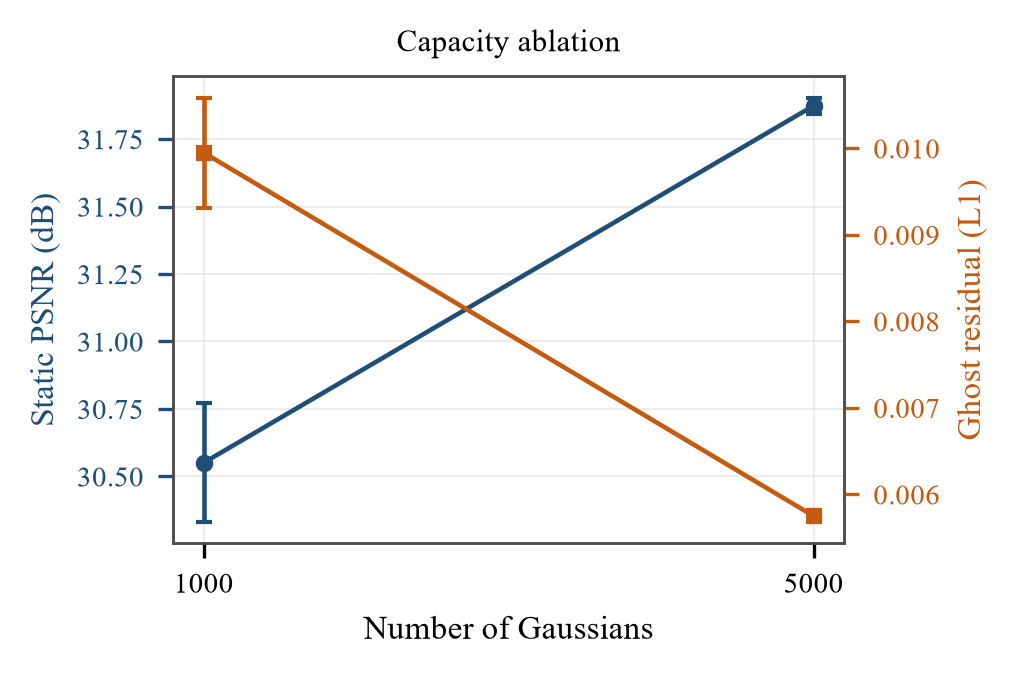
\includegraphics[width=0.48\textwidth]{ablation_points.png}
\caption{Capacity ablation. Static-region PSNR and dynamic ghost residual as the number of Gaussian primitives is varied, with the optimization budget, mask, and seeds held fixed.}
\label{fig:ablpts}
\end{figure}

Fig.~\ref{fig:abliter} isolates the schedule. The budget sweep evaluates only the combined masked configuration. Its improvement with additional iterations is a within-configuration result; baseline comparisons at 600 and 2,400 iterations remain unmeasured.

\begin{figure}[t]
\centering
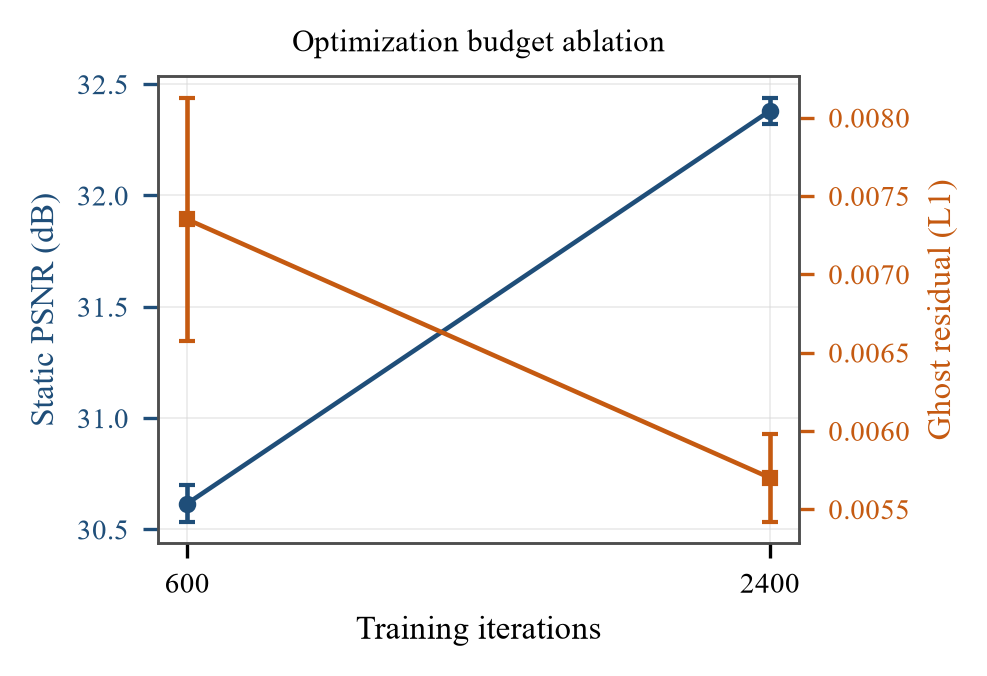
\includegraphics[width=0.48\textwidth]{ablation_iters.png}
\caption{Optimization-budget ablation. The combined masked configuration at two additional training budgets. The other configurations were not evaluated at the two additional budgets.}
\label{fig:abliter}
\end{figure}

Fig.~\ref{fig:noise} replaces the perfect oracle with a deliberately corrupted one. The observed static-region PSNR is 31.59, 31.61, and 31.55 dB at 5, 10, and 20 percent label-flip rates. This response is small and non-monotone. Noise is resampled during optimization and affects the loss mask while initialization retains oracle labels. It therefore measures stochastic loss-mask corruption, rather than a fixed erroneous segmentation front end.

\begin{figure*}[t]
\centering
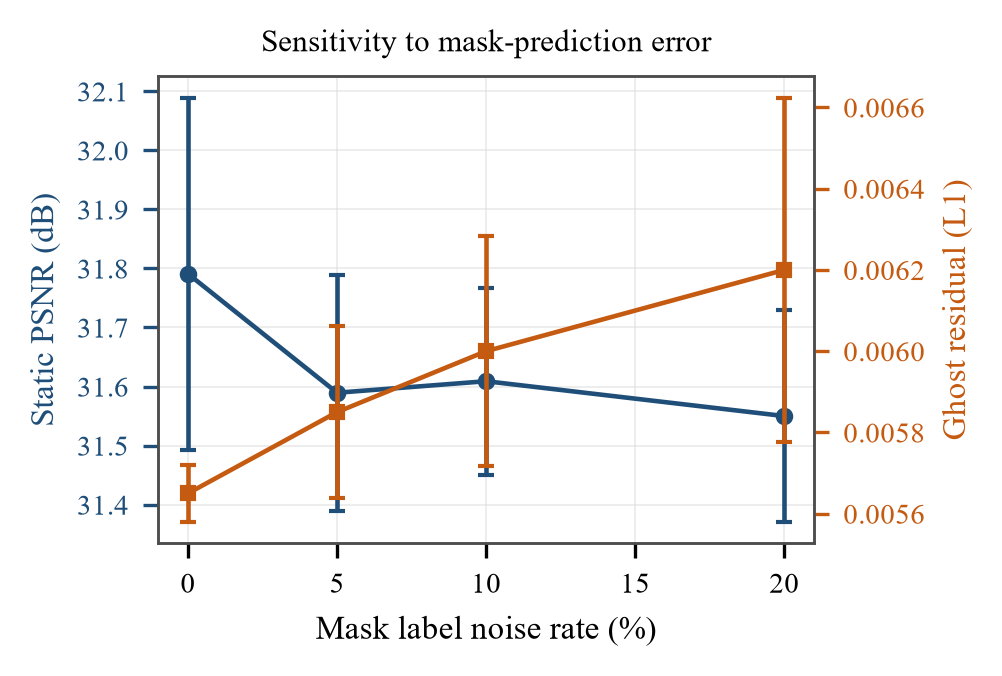
\includegraphics[width=0.60\textwidth]{mask_noise_sensitivity.png}
\caption{Sensitivity to mask-label noise. Ground-truth dynamic labels are flipped at a controlled rate before the mask is applied. Noise is resampled per optimization step; these results do not establish performance with a real mask predictor.}
\label{fig:noise}
\end{figure*}




\subsection{Separating initialization from loss masking}
The original three configurations leave one causal question unresolved: whether loss masking alone recovers the benefit without static-only initialization. We add this fourth configuration with seeds 0, 1, and 2. All observations can initialize the map, while the loss uses the oracle static-validity mask. The training split, 2,500 primitives, 1,200 iterations, and four held-out views match the other configurations. Table~\ref{tab:newruns} and Fig.~\ref{fig:newruns} compare the common three-seed subset; the five-seed main table remains a separate summary.

Loss-only masking reaches $30.986\pm0.066$ dB and a ghost residual of $0.0057\pm0.0005$. Initialization plus loss masking reaches $31.647\pm0.217$ dB and $0.0058\pm0.0003$, respectively. The combined intervention improves static-region fidelity over loss masking alone, but their ghost residuals are close. Thus loss masking accounts for much of the transient-suppression effect in this scene, while initialization filtering supplies an additional static-fidelity benefit. These measurements do not support a claim that both stages are necessary to minimize every metric.

\begin{table}[t]
\centering\scriptsize
\caption{Matched three-seed intervention and fixed mask-error tests. Mean and sample SD; evaluated with uncorrupted held-out masks.}
\label{tab:newruns}
\begin{tabular}{lcc}\toprule
Configuration & Static PSNR & Ghost L1 \\
\midrule
All pixels & $27.899\pm0.281$ & $0.0383\pm0.0045$ \\
Initialization only & $29.338\pm0.548$ & $0.0270\pm0.0103$ \\
Loss only & $30.986\pm0.066$ & $0.0057\pm0.0005$ \\
Initialization + loss & $31.647\pm0.217$ & $0.0058\pm0.0003$ \\
20\% false negatives & $31.504\pm0.197$ & $0.0065\pm0.0003$ \\
20\% false positives & $31.561\pm0.033$ & $0.0059\pm0.0001$ \\
\bottomrule\end{tabular}
\end{table}

\begin{figure*}[t]
\centering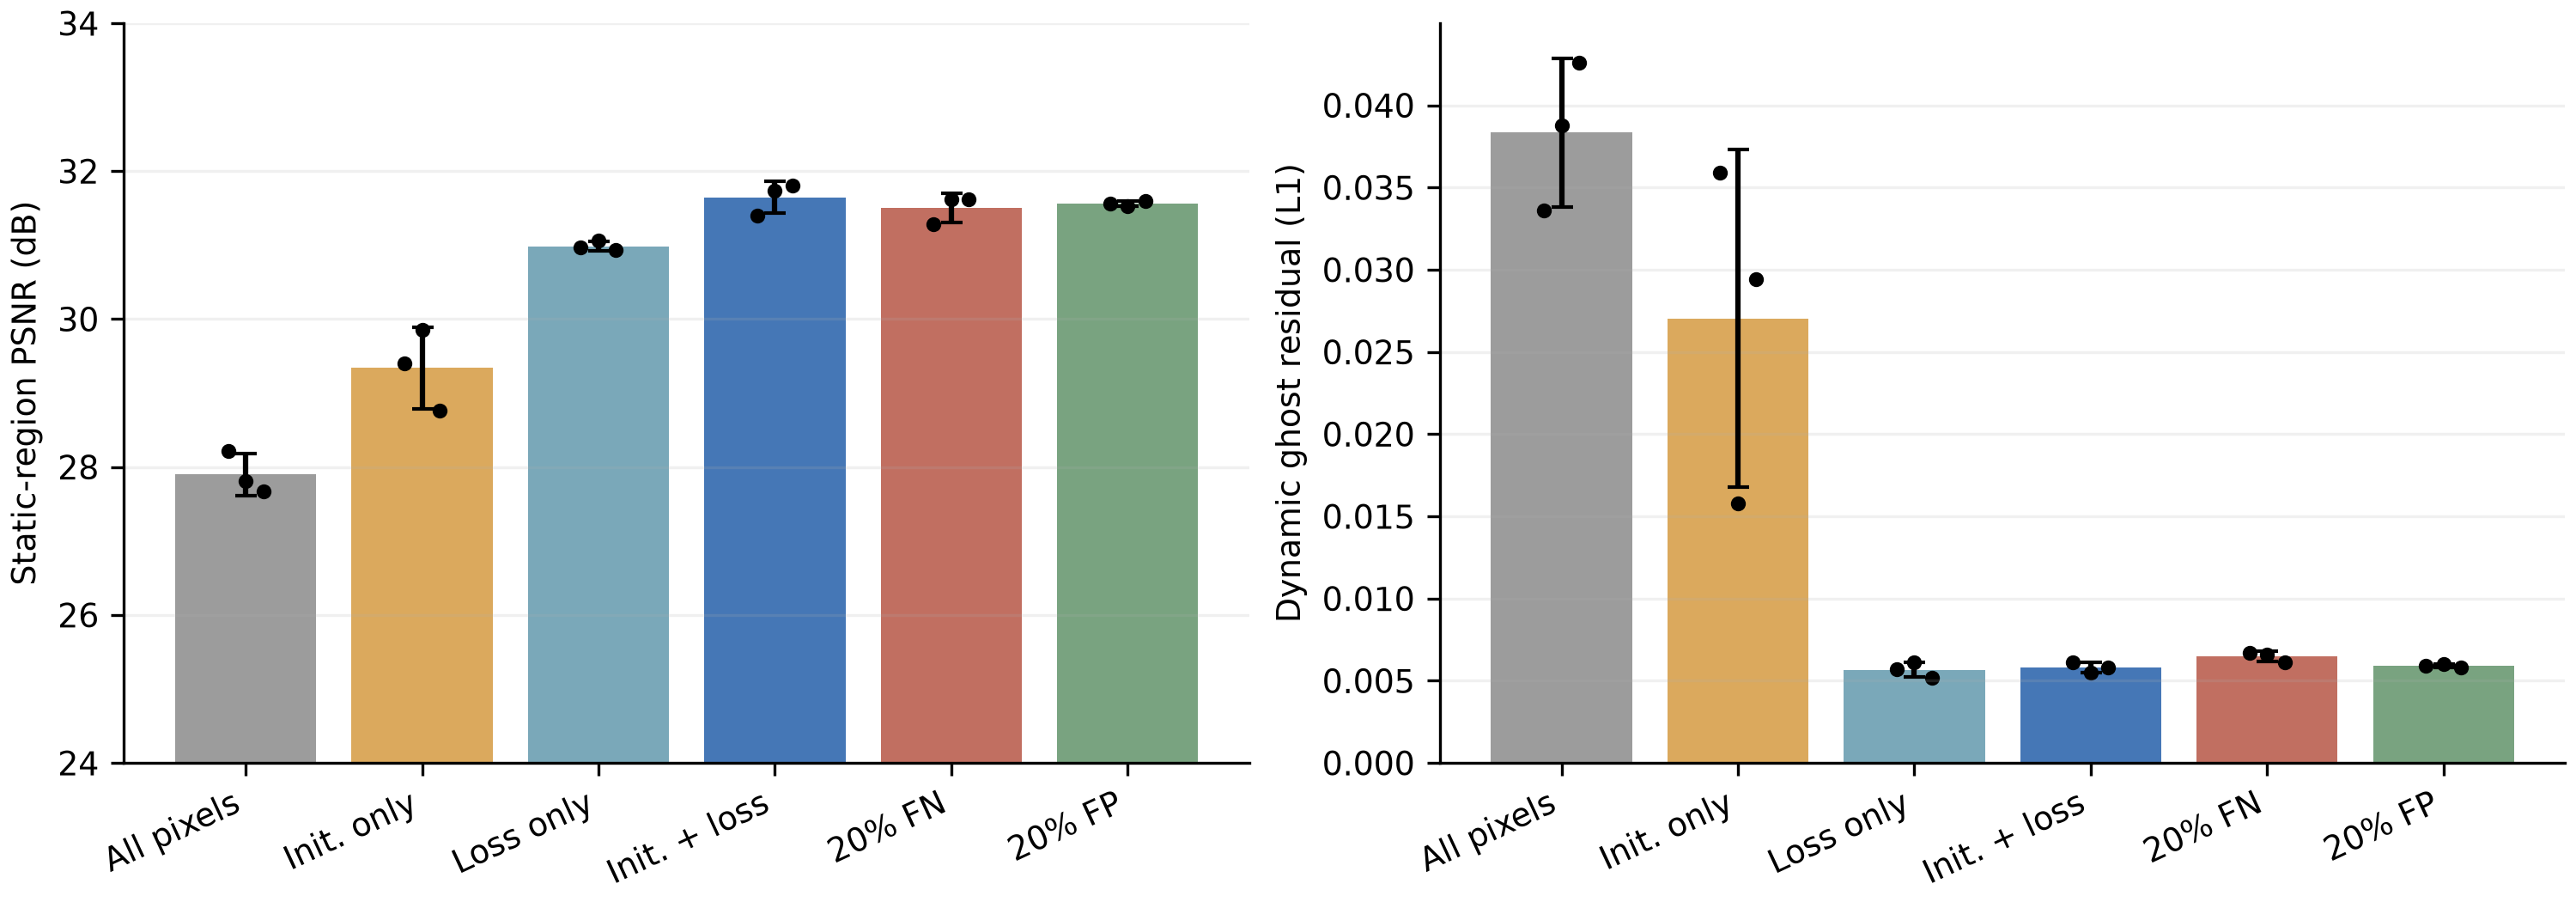
\includegraphics[width=.94\textwidth]{matched_interventions.png}
\caption{Matched-seed intervention and mask-error results. Points are individual runs and bars show means with sample SD. The three-seed comparison uses identical training budgets and held-out views.}
\label{fig:newruns}
\end{figure*}

\subsection{Fixed false-negative and false-positive masks}
The earlier label-flip sweep resamples random corruption during optimization and leaves initialization clean. We additionally test fixed masks shared by initialization and loss. A false-negative trial independently changes each dynamic pixel to static with probability 0.2. A false-positive trial independently changes each static pixel to dynamic with probability 0.2. Realized class-conditional rates range from 19.07\% to 20.06\% across the six runs. These are class-conditional rates: because the classes occupy different image areas, they are not equal fractions of all pixels. The sampled masks are held fixed for all iterations in a run; ground-truth held-out masks are retained for evaluation.

False-negative corruption yields $31.504\pm0.197$ dB with ghost residual $0.0065\pm0.0003$, and false-positive corruption yields $31.561\pm0.033$ dB with residual $0.0059\pm0.0001$. This directly measures two distinct mechanisms: leaked dynamic observations can contaminate the map, whereas discarded static observations reduce support. The outcome remains conditional on independent pixel errors and a small synthetic scene. Spatially coherent segmentation failures, incorrect poses, and real image noise are not reproduced by this test.

\begin{figure*}[t]
\centering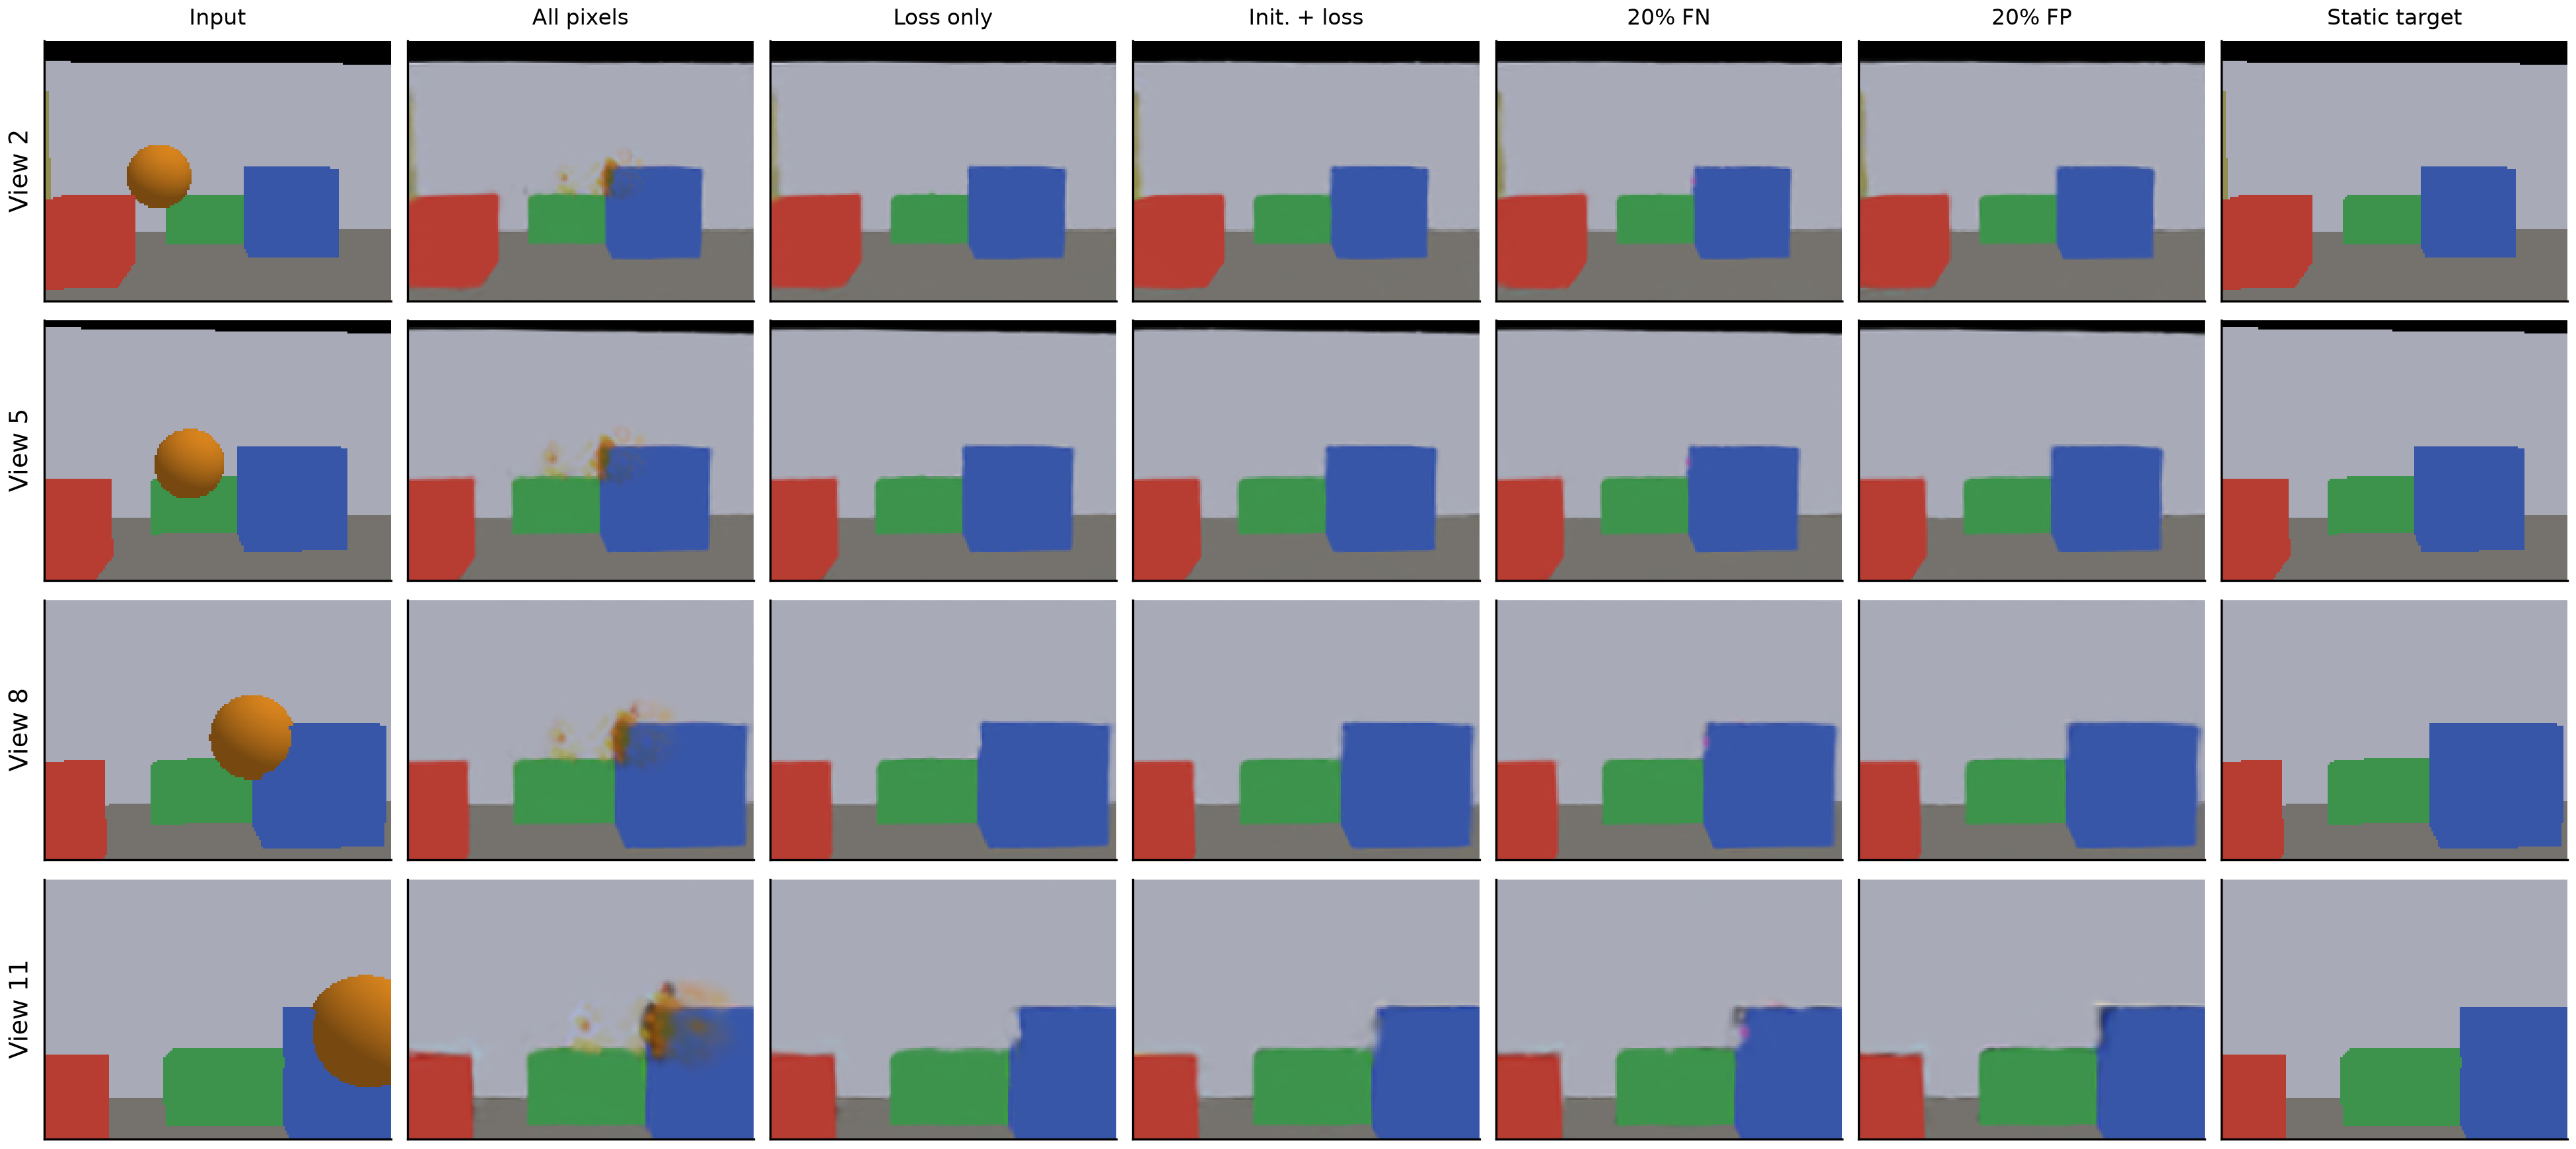
\includegraphics[width=.98\textwidth]{new_gpu_renders.png}
\caption{GPU-rendered held-out comparisons for seed 0. Every declared held-out view is shown. Columns use the same camera and native $160\times120$ arrays; nearest-neighbor enlargement is used for display. The clean target excludes the moving object.}
\label{fig:newrenders}
\end{figure*}

\begin{figure*}[t]
\centering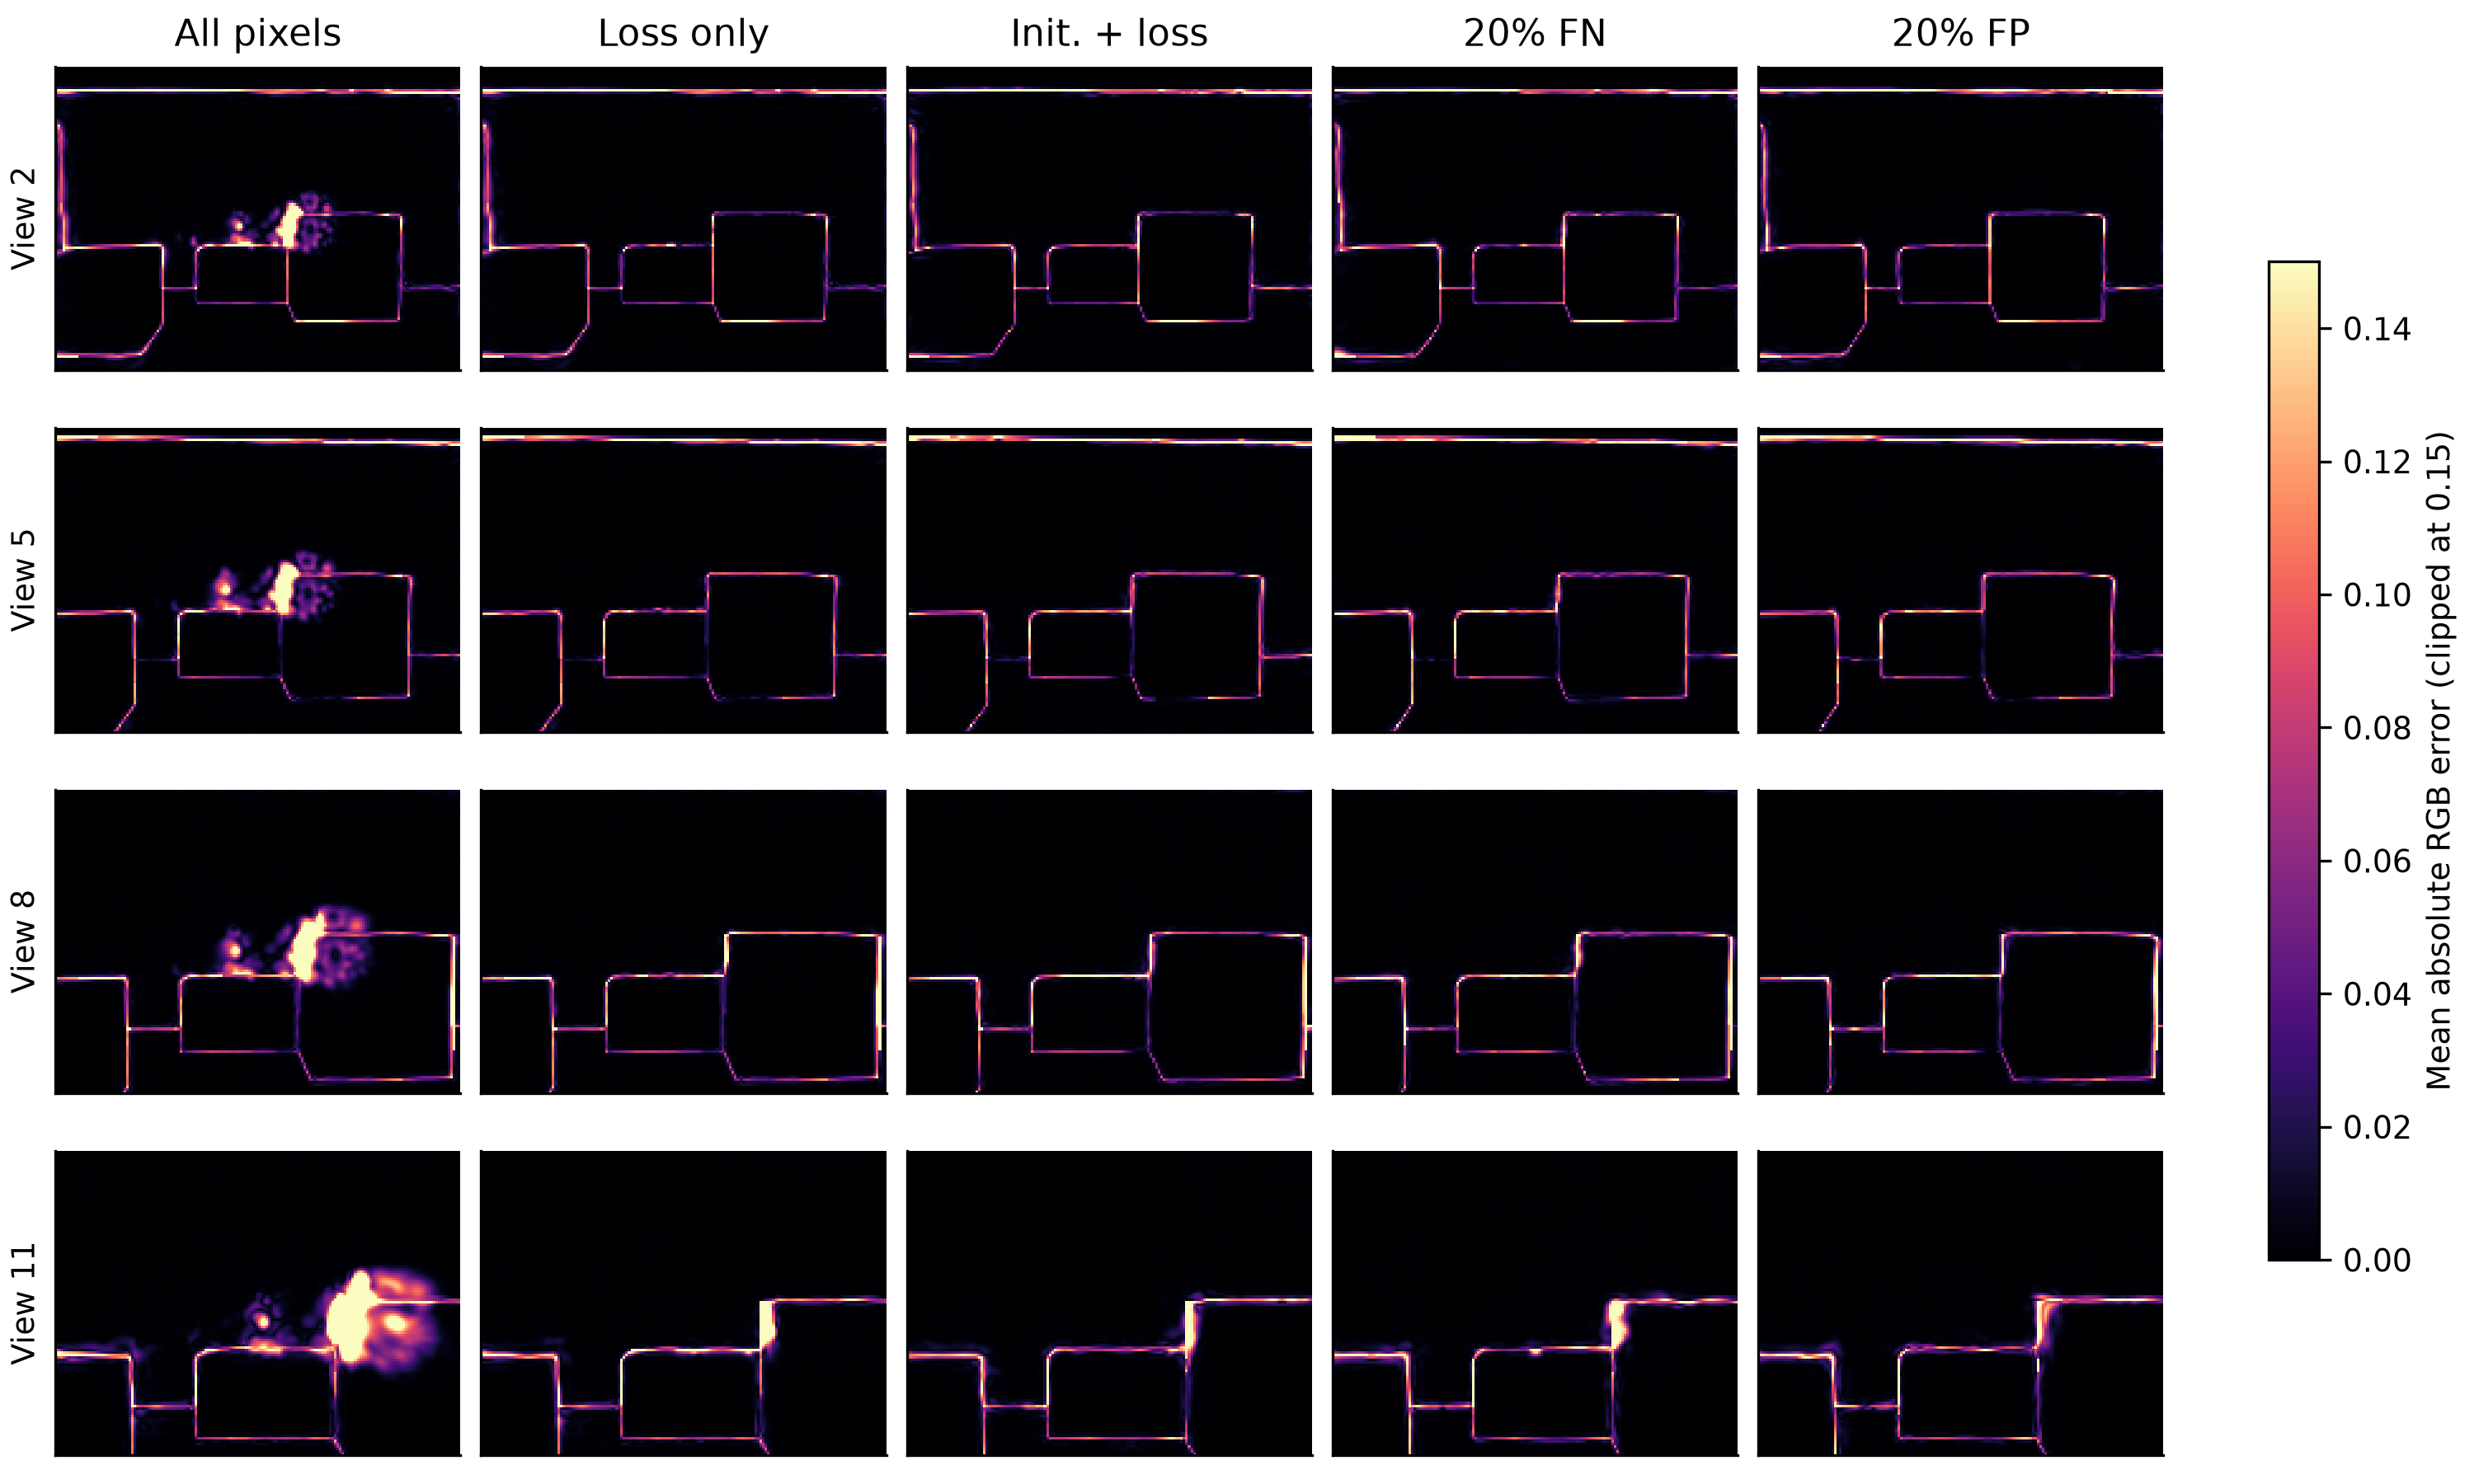
\includegraphics[width=.94\textwidth]{new_error_maps.png}
\caption{Per-pixel mean absolute RGB error against the static target for the same held-out views and seed. All panels share the color scale, clipped at 0.15 for visibility. Clipping applies only to the plotted color range; reported metrics use the unclipped arrays.}
\label{fig:newerrors}
\end{figure*}

\subsection{Reading the rendered comparisons}
Figures~\ref{fig:newrenders} and~\ref{fig:newerrors} connect aggregate values to the underlying pixels. The input column contains the moving foreground, whereas the static target defines the persistent-map objective. A renderer that accurately reproduces the foreground can therefore have a lower dynamic-input error and a higher ghost residual at the same time. This is why whole-image fidelity to the observed frame is insufficient for assessing static-map contamination.

All four held-out views are displayed in their declared order. The error maps use one color scale so that an apparent improvement cannot result from independently rescaling each panel. The visualizations are produced from saved float arrays; the artifact additionally retains the original model checkpoints and newly rendered baseline arrays. The native resolution limits the fine geometry that can be assessed, and enlargement adds no spatial information. The figure should therefore be read as a comparison of contamination patterns and static support, not as evidence of high-resolution reconstruction quality.

The individual run points also matter. With only three seeds, a small difference in the mean ghost residual should not be treated as a general ranking. The stable result is the separation between unmasked training and loss-masked configurations; the residual distinction among well-masked configurations is much smaller. Reporting both individual runs and per-view panels exposes this scale difference and avoids interpreting every visible bar separation as a meaningful system advantage.

\section{Discussion}
\subsection{What the two experiments jointly establish}
The fusion and mapping experiments test different interfaces. The first shows that a provenance-aware pool passes an exact-duplication sanity check. The second shows that correct dynamic suppression must remain active during optimization, not merely at initialization. Together they support a design principle: uncertainty should be controlled both when evidence is combined and when that evidence weights the map update.

They do not show that the family pool produces better masks on a real sequence. A learned front end could be poorly calibrated, the assigned families could be wrong, or geometry could fail under pose error. Similarly, the oracle mapping gain is an upper-bound style diagnostic: a practical mask will contain false positives and false negatives, and those errors can change the ordering.

\subsection{Relation to Dy3DGS-SLAM}
Li et al. already describe a dynamic Gaussian SLAM system that uses optical flow, depth-related information, and dynamic mapping losses \cite{li2025dy3dgs}. Our title and claims therefore avoid the same-name system framing. The substantive difference studied here is whether channels derived from a common source receive a fixed total evidential budget and whether that property can be audited by replication. This is complementary to, rather than a replacement for, the full pipeline in Dy3DGS-SLAM.

A future comparative experiment must run both systems or faithfully reproduce their public implementations under matched data, camera inputs, alignment, and hardware. Citing another paper's result table is related-work context, not experimental evidence for the present method.

\subsection{When family pooling may not help}
If all channels are independently measured and well calibrated, a correctly specified likelihood model can exploit more information than a family mean. If one family is systematically better, uniform family weights may underweight it. If a family contains one strong channel and several weak transformations, averaging can dilute the strong signal. These cases motivate validation-learned weights or a hierarchical probabilistic model.

The proposed rule is most useful when provenance is known but the full dependence structure is not reliably estimable. It is a conservative guard against representation-driven confidence. It should be compared against logistic stacking, covariance-aware fusion, learned gating, and ablations of family assignment on real sequences.

\subsection{Mask error propagation}
False-negative dynamic pixels enter the static map and can create ghosts. False-positive dynamic pixels remove useful static constraints, potentially producing holes or weakening tracking. A soft probability can reduce discontinuity but may still give a high-residual moving object enough gradient to contaminate the map. A complete evaluation should sweep thresholds, perturb masks with controlled false-positive/false-negative rates, and report both map quality and tracking failure.

\subsection{Interpretation of the synthetic scene}
The simple scene is a strength for mechanism isolation and a weakness for external validity. It contains known geometry, a single moving object, and clean oracle annotations. It does not include articulated motion, specular surfaces, textureless areas, rolling shutter, motion blur, depth discontinuities typical of real sensors, or long-term loop closure. The observed 3.75 dB gain should therefore not be projected onto TUM, BONN, Replica, or in-the-wild sequences.

\section{Limitations, Threats, and Responsible Reporting}
\subsection{Internal validity}
The mapping runs use fixed data and three seeds. They are reproducible but do not characterize sensitivity to learning rates, Gaussian count, densification, or scene geometry. The SSIM implementation is an inherited box-window variant and may not match another paper's library settings. Timing is wall-clock on one workstation and is affected by warm-up and background activity.

The stress test uses a designed latent-variable generator. It validates algebraic and numerical behavior under exact replication but does not establish the correlation structure of real optical-flow, depth, and clustering outputs. ECE depends on ten bins; NLL and Brier are included to prevent the conclusion from resting on one binned metric.

\subsection{External validity}
Ground-truth poses remove tracking drift, and ground-truth depth removes monocular scale ambiguity. Oracle masks remove segmentation errors. Consequently, the experiment cannot support ATE, RPE, mask F1/IoU, loop closure, failure rate, or metric-scale claims. Real-sequence evaluation must include TUM RGB-D dynamic sequences and BONN dynamic scenes, while a rendering study can include Replica with a declared train/test split.

\subsection{Comparison validity}
Different Gaussian SLAM papers use different sensors, alignment rules, hardware, image resolutions, and metric implementations. A comparison table is meaningful only when these conditions are explicit. In particular, monocular trajectories aligned by $Sim(3)$ cannot be interpreted as evidence of metric scale recovery. Runtime comparisons must state whether segmentation, depth, flow, tracking, mapping, and rendering are included.

\subsection{Reproducibility and AI assistance}
The artifact records source and data hashes, split indices, seeds, environment versions, per-frame metrics, model files, Gaussian point clouds, and rendered outputs. An AI assistant helped audit the original manuscript, implement the controlled analyses, and edit prose. The authors remain responsible for checking the code, authorship, citations, experimental claims, and the final venue's disclosure policy. No AI-generated number is treated as evidence unless it is backed by the stored experiment output.

\subsection{Potential misuse}
Dynamic-object suppression can remove people or objects from a map. That may be useful for privacy and static navigation, but it can also erase safety-relevant agents or encode dataset bias. A deployed robot should maintain a separate dynamic-world representation for collision avoidance rather than equating ``excluded from the static map'' with ``irrelevant.'' Data collection must respect privacy and benchmark licenses.

\section{Required End-to-End Validation}
A complete submission-level system evaluation should implement the following protocol.

\textbf{Mask prediction.} Generate flow, depth, and derived clustering channels on real images. Calibrate them on held-out sequences, not frames sampled from the test trajectory. Report IoU, precision, recall, F1, NLL, Brier, ECE, reliability plots, and threshold sensitivity. Include product, channel mean, family pool, learned stacking, and single-family baselines.

\textbf{Tracking.} Run the full camera tracker and report ATE RMSE, RPE translation/rotation, failure rate, and successful-frame fraction. Declare $SE(3)$ versus $Sim(3)$ alignment and whether scale comes from RGB-D input, an external metric-depth model, or post-hoc alignment. Use multiple runs when stochastic components affect the trajectory.

\textbf{Mapping.} Evaluate held-out PSNR, SSIM, LPIPS, depth error, and static-map ghost measures. Separate novel-view quality from reconstruction of the dynamic input image. Include mask-noise sweeps and an ablation that applies masks only during initialization, only during optimization, and at both stages.

\textbf{Baselines.} Compare with the existing Dy3DGS-SLAM \cite{li2025dy3dgs}, DG-SLAM \cite{xu2024dg}, WildGS-SLAM \cite{zheng2025wildgs}, GARAD-SLAM \cite{li2025garad}, and appropriate static Gaussian baselines \cite{matsuki2024,keetha2024splatam}. Use official code and checkpoints where possible, record commit hashes, and avoid mixing numbers from incompatible protocols.

\textbf{Efficiency.} Synchronize GPU timing, include warm-up, and report median and tail latency for flow, depth, segmentation/fusion, tracking, mapping, and rendering. Report peak allocated and reserved memory. End-to-end FPS is the reciprocal of the full critical path, not of an isolated renderer.

This protocol is not reported as completed work. It is the explicit evidence needed before the mechanism study can support a full SLAM claim.

\section{Conclusion}
Derived vision channels do not become independent evidence merely because they occupy separate feature slots. In the controlled stress test, a fixed product becomes severely overconfident when one motion observation is copied, while a source-family logit pool remains invariant. In the separate mapping study, static-only initialization helps, but loss masking supplies most of the observed transient suppression, while initialization filtering further improves static-region fidelity. The verified contribution is therefore a provenance-aware fusion sanity property and an isolated mapping ablation. Real-image mask quality, monocular scale, tracking accuracy, and end-to-end robustness remain to be demonstrated under the stated validation protocol.


\appendices
\section{Reproducibility Details}
All mapping runs use the fixed eight-view training split and four held-out views specified in the experimental protocol. The artifact retains per-run metrics, random seeds, optimization histories, model parameters, and original rendered outputs. The main experiment has five seeds per configuration. Capacity, budget, and label-flip sweeps have two seeds per setting; morphology checks have one run and therefore provide no estimate of run-to-run variation. Additional intervention and class-conditional mask-error tests use three matched seeds. Mean and sample standard deviation are reported where at least two runs are available; a one-run result is reported without a standard deviation.

Figures use the stored output arrays, shared axes, and common error-map limits. Crops are identified in their captions. Enlarged renderings use nearest-neighbor display; no image synthesis or content retouching is applied. Image panels retain the original synthetic-scene resolution of $160\times120$. The release contains the numeric arrays needed to reproduce plots independently of document formatting.

\bibliographystyle{IEEEtran}
\bibliography{references}
\end{document}
